\documentclass[11pt,a4paper]{article}

\usepackage[a4paper,margin=1in]{geometry}
\usepackage{booktabs}
\usepackage{array}
\usepackage{tabularx}
\usepackage{longtable}
\usepackage{graphicx}
\usepackage{caption}
\usepackage{subcaption}
\usepackage{xcolor}
\usepackage{hyperref}
\usepackage{amsmath,amssymb}
\usepackage{float}
\usepackage{natbib}
\usepackage{url}

\hypersetup{
  colorlinks=true,
  linkcolor=blue!50!black,
  citecolor=blue!50!black,
  urlcolor=blue!50!black
}

\graphicspath{
  {../../exp/v5.2/0_tokenizer/03_tokenization_effect/}
  {../../exp/v5.2/Plot/loss/}
  {../../exp/v5.2/2_training/}
  {../../exp/v5.2/3_evaluation/09_family_similarity/}
  {../../exp/v5.2/4_reporting/}
  {../tex_ko/figs/}
}

\newcommand{\todo}[1]{\textcolor{red}{[TODO: #1]}}
\DeclareRobustCommand{\codepath}[1]{\path{#1}}
\newcommand{\method}[1]{\textsc{#1}}
\newcommand{\rand}{\texttt{random}}
\newcommand{\meanm}{\texttt{mean}}
\newcommand{\fvt}{\texttt{fvt}}
\newcommand{\wfvt}{\texttt{weighted\_fvt}}
\newcommand{\famm}{\texttt{family\_mean}}
\newcommand{\dn}{$\downarrow$}
\newcommand{\up}{$\uparrow$}

\title{XLM-R-Based Glot500-Style Vocabulary Extension for Low-Resource Tail Languages}
\author{Jongha Kim \\
Sogang University}
\date{NLP Term Project \\ July 4, 2026}

\begin{document}
\maketitle

\begin{abstract}
본 보고서는 Glot500의 horizontal scaling 방향을 작은 재현 가능한 설정으로 가져와,
XLM-R 기반 multilingual encoder를 low-resource tail language로 확장할 때 새 vocabulary
embedding row의 초기화가 얼마나 중요한지 분석한다. 실험은 92개의 XLM-R-seen
language-script와 downstream 평가가 가능한 7개의 XLM-R-unseen target language-script를
사용한다. Tokenizer는 Glot500과 같이 mixed corpus에서 SentencePiece unigram tokenizer를
학습하고 기존 XLM-R SentencePiece model 뒤에 새 piece를 append하는 방식으로 고정한다.
따라서 main ablation은 tokenizer 자체가 아니라 새 token embedding row의 initialization,
즉 \method{random}, \method{mean}, \method{FVT}, \method{weighted FVT},
\method{family-aware mean}의 차이다.

최종 보고서는 50K-step convergence run을 중심으로 다섯 초기화 방법의 training loss,
pseudoperplexity, downstream scores를 tail/head/all group으로 정리한다. Step-4000 결과는
수렴 결과가 아니라 early diagnostic evidence로만 사용한다. 이 구분은 중요하다. 4K 이하
checkpoint에서는 \method{FVT}가 target pseudoperplexity와 여러 retrieval/alignment task에서
강한 초기 신호를 보였지만, 최종 주장은 50K run에서 loss flattening과 downstream trajectory가
확인된 뒤에만 세운다. 따라서 본 보고서는 특정 initialization이 모든 task에서 항상 최고라고
주장하지 않는다. 대신 같은 tokenizer, corpus, MLM objective, evaluation protocol을 공유하는
controlled setup에서 새 token embedding initialization이 low-resource vocabulary adaptation의
수렴 양상과 평가 지표에 실질적인 영향을 주는지를 검증한다.
\end{abstract}

\section{Introduction}

Advances in large language models have proceeded along two axes.
\textbf{Vertical scaling} deepens understanding of a fixed set of high-resource languages
by increasing parameter count, training data, and compute---ChatGPT, Claude, and scaling-law
research belong here.
\textbf{Horizontal scaling} asks instead whether a model can support more languages,
domains, and tasks.
Supporting low-resource tail languages is the canonical horizontal-scaling problem and
is the background of this report.
XLM-R \citep{conneau2020xlmr} is a strong multilingual encoder, but for languages
absent from its training data it suffers from two compounding deficits:
(1)~token over-fragmentation, where a single morpheme is split into many subword pieces,
and (2)~representation mismatch, where the embedding space carries no signal from
the target language.

Glot500 \citep{imani2023glot500} combines vocabulary extension with continued MLM
pretraining to address these deficits for 511 language-scripts.
After extending the tokenizer, XLM-R's embedding matrix $\mathbf{E}\in\mathbb{R}^{250002\times768}$
grows to $\mathbb{R}^{366666\times768}$: the 116,664 new rows have never received a gradient.
Glot500 initializes these rows randomly.
Whether a different starting point---one that reuses information already encoded in
the existing XLM-R embeddings---leads to better convergence and downstream performance
under a limited training budget is the question this report addresses.

We investigate three research questions:
\begin{enumerate}
  \item Does Glot500-style SentencePiece append reduce subword fragmentation for
        XLM-R-unseen tail languages?
  \item With tokenizer and corpus held fixed, does changing only the initialization of
        new token rows alter PPPL and downstream task scores?
  \item Does the sentence representation space exhibit language-identity or
        family/typology structure after continued pretraining?
\end{enumerate}

This experiment is not a full reproduction of Glot500 across 511 languages.
All seven Target7 languages use Latin script, so we make no claim about script diversity.
Instead, we select the smallest XLM-R-unseen tail-language corpus band that still
supports downstream evaluation, and run a controlled 5-way initialization ablation
with identical tokenizer, corpus, objective, schedule, and evaluation protocol.

Our contributions are:
\begin{enumerate}
  \item We propose \famm, a family-aware initialization that places new token rows
        at the centroid of source embeddings belonging to the same language family,
        and verify it against four baselines (\rand, \meanm, \fvt, \wfvt) in a
        controlled 5-way ablation with the tokenizer fixed.
  \item We connect the 2D similarity map's family clustering with downstream results,
        showing that family-aware initialization converges to the best target PPPL,
        Tatoeba retrieval, and NER scores.
  \item We track the step-by-step formation of family geometry in the representation
        space and use it to interpret why family-prior initialization reaches a better
        optimum.
\end{enumerate}

\section{Related Work}

\subsection{Glot500 and Horizontal Scaling}

Glot500은 XLM-R이 지원하는 약 100개 언어를 head language로, 그 밖의 언어를 tail
language로 정의하고, multilingual model의 horizontal scaling을 제안한다
\citep{imani2023glot500}. 원 논문은 language-script 단위 corpus cleaning, 30,000
sentence' 이상 기준, SentencePiece unigram tokenizer 재학습, XLM-R vocabulary 확장,
continued MLM pretraining을 하나의 pipeline으로 구성한다. Glot500-m은 XLM-R vocabulary
250K에 약 151K new token을 추가해 401K vocabulary를 만들고, 600GB corpus에서 MLM으로
continued pretraining한다.

원 논문 Table 4는 Glot500-m이 tail group에서 특히 큰 개선을 보인다고 보고한다. 본
보고서에서는 그 표를 단순 baseline으로 가져오는 데 그치지 않고, 왜 본 실험이 같은
head/tail/all reporting structure를 따라야 하는지의 근거로 사용한다.

\begin{table}[t]
\centering
\caption{Glot500 original head/tail/all reference table from \citet{imani2023glot500}. Values are averages across five seeds; retrieval, tagging, classification, and roundtrip values are percentages.}
\label{tab:glot500-reference}
\resizebox{\textwidth}{!}{%
\begin{tabular}{lrrrrrrrrr}
\toprule
 & \multicolumn{3}{c}{tail} & \multicolumn{3}{c}{head} & \multicolumn{3}{c}{all} \\
\cmidrule(lr){2-4}\cmidrule(lr){5-7}\cmidrule(lr){8-10}
Metric & XLM-R-B & XLM-R-L & Glot500-m & XLM-R-B & XLM-R-L & Glot500-m & XLM-R-B & XLM-R-L & Glot500-m \\
\midrule
Pseudoperplexity & 304.2 & 168.6 & 12.2 & 12.5 & 8.4 & 11.8 & 247.8 & 136.4 & 11.6 \\
Sentence Retrieval Tatoeba & 32.6 & 33.6 & 59.8 & 66.2 & 71.1 & 75.0 & 56.6 & 60.4 & 70.7 \\
Sentence Retrieval Bible & 7.4 & 7.1 & 43.2 & 54.2 & 58.3 & 59.0 & 19.3 & 20.1 & 47.3 \\
Text Classification & 13.7 & 13.9 & 46.6 & 51.3 & 60.5 & 54.7 & 23.3 & 25.8 & 48.7 \\
NER & 47.5 & 51.8 & 60.7 & 61.8 & 66.0 & 63.9 & 55.3 & 59.5 & 62.4 \\
POS & 41.7 & 43.5 & 62.3 & 76.4 & 78.4 & 76.0 & 65.8 & 67.7 & 71.8 \\
Roundtrip Alignment & 2.6 & 3.1 & 4.5 & 3.4 & 4.1 & 5.5 & 2.8 & 3.3 & 4.7 \\
\bottomrule
\end{tabular}}
\end{table}


\subsection{SentencePiece Unigram and Vocabulary Extension}

SentencePiece는 library 이름이고, 그 안에서 BPE 또는 unigram language model을 사용할 수
있다 \citep{kudo2018sentencepiece}. XLM-R과 Glot500은 SentencePiece unigram 계열을 사용한다.
Unigram LM은 가능한 subword 후보 집합을 크게 시작한 뒤, EM으로 token probability를
추정하고 likelihood contribution이 낮은 token을 pruning하는 top-down 방식이다. 이 선택은
BPE처럼 greedy merge만 누적하는 방식과 달리 여러 segmentation 후보를 확률적으로 다룬다.

본 프로젝트의 tokenizer는 이 Glot500 흐름을 따른다. \codepath{tokenization/run.py}는
\codepath{--model_type=unigram}, \codepath{--byte_fallback=true},
\codepath{--character_coverage=1.0}으로 새 SentencePiece model을 학습하고, 기존 XLM-R
SentencePiece protobuf에 없는 piece만 append한다.

\subsection{Embedding Initialization for New Tokens}

Vocabulary expansion 연구에서는 새 token을 추가한 뒤 embedding을 어떻게 초기화할지가
중요하다. Yamaguchi et al.은 30K sentences, 약 0.01GB target language text만 있는
low-resource setting에서 vocabulary expansion과 target parameter initialization을 비교하고,
high-resource에서 자주 쓰이는 random initialization이 항상 최선이 아니라고 보고한다
\citep{yamaguchi2025vocab}. Mean initialization은 기존 embedding centroid를 사용하고,
FVT 계열은 새 token surface를 source tokenizer로 다시 분해한 뒤 source subtoken embedding을
평균한다 \citep{hewitt2021newembeddings,vocabextensiontutorial2026}.

본 연구는 decoder LLM이 아니라 XLM-R encoder 기반 MLM setting이지만, 질문은 같다. 새
token row를 완전히 무작위로 시작할지, 기존 XLM-R tokenizer와 embedding space가 이미 가진
표면형 정보를 재사용할지 비교한다.

\section{Data}

\subsection{Target Definition}

v5.2의 corpus universe는 `99` language-script이다. 이 중 `92`개는 XLM-R training language로
표시된 seen/head language이고, `7`개는 XLM-R-unseen target tail language이다. 초기 feedback은
``low-resource language를 task별 3개씩 포함하도록 고른 이유''를 더 명확히 요구했다. 이에
따라 target은 단순히 가장 작은 corpus가 아니라 다음 조건으로 정의한다.

\begin{quote}
XLM-R-unseen tail languages in the smallest Glot500 corpus band that still supports downstream evaluation.
\end{quote}

strict `new\_length <= 10k` non-XLM-R tail language는 local task-list membership이 없어
Tatoeba, Bible, NER, POS 등을 3개씩 채울 수 없다. 따라서 downstream evidence를 확보하기
위해 약 30K--50K Glot500 sentence' band에서 task overlap이 가장 큰 7개 언어를 선택했다.
이 결정은 \codepath{docs/exp/v5.2/1_data_scope/low_resource_task_fill_candidates_ko.md}와
\codepath{preprocessing/prepare_v5_glot50010_merge_inputs.py}의
\codepath{V52_OVERLAP_TASKFILL_GLOT5007}에 기록되어 있다.

\begin{table}[t]
\centering
\caption{Target7 selection. All target languages are XLM-R-unseen Glot500 raw languages with at least 30,000 sentence' units and useful downstream overlap.}
\label{tab:target7}
\resizebox{\textwidth}{!}{%
\begin{tabular}{llllrl}
\toprule
language-script & full name & region & script & new\_length & covered tasks \\
\midrule
dtp\_Latn & Kadazan Dusun & Southeast Asia & Latn & 48,468 & Tatoeba, Bible, Roundtrip, Taxi1500, Embedding similarity \\
xav\_Latn & Xavante & South America & Latn & 31,765 & Bible, Roundtrip, POS, Taxi1500 \\
bam\_Latn & Bambara & West Africa & Latn & 32,150 & Bible, Roundtrip, POS, Taxi1500 \\
csb\_Latn & Kashubian & Europe & Latn & 33,743 & Tatoeba, NER, Embedding similarity \\
ile\_Latn & Interlingue & Constructed/Europe & Latn & 40,984 & Tatoeba, Embedding similarity \\
lij\_Latn & Ligurian & Europe & Latn & 42,447 & NER, POS \\
fur\_Latn & Friulian & Europe & Latn & 30,052 & NER \\
\bottomrule
\end{tabular}}
\end{table}


\subsection{Task Coverage}

Target7은 총 21개 task slot을 7개 언어로 압축한다. 이 표는 왜 downstream task를 사용할 수
있는지, 그리고 어떤 결과를 target evidence로 말할 수 있는지의 근거이다.

\begin{table}[t]
\centering
\caption{Downstream coverage rationale for Target7. This table is the defense artifact for why the target set is not the strict smallest corpus set.}
\label{tab:task-coverage}
\begin{tabularx}{\textwidth}{lXl}
\toprule
Task & target languages & current status \\
\midrule
Tatoeba retrieval & csb\_Latn, dtp\_Latn, ile\_Latn & ready local pairs \\
Bible retrieval & dtp\_Latn, xav\_Latn, bam\_Latn & materialized parallel verses \\
Roundtrip alignment & dtp\_Latn, xav\_Latn, bam\_Latn & Bible-derived JSONL \\
NER & csb\_Latn, lij\_Latn, fur\_Latn & PAN-X train/dev/test ready \\
POS & xav\_Latn, bam\_Latn, lij\_Latn & rebuilt/materialized split \\
Taxi1500 & dtp\_Latn, xav\_Latn, bam\_Latn & not target7 evidence in current draft \\
Embedding similarity & csb\_Latn, dtp\_Latn, ile\_Latn & diagnostic pairs ready \\
\bottomrule
\end{tabularx}
\end{table}


\subsection{Training Corpus}

MLM training corpus는 \codepath{preprocessing/run_v52_glot5007_merge.sh}가
\codepath{preprocessing/merge_files.py}를 호출하여 만든다. Sampling은 Glot500-style language
sampling factor $\alpha=0.3$을 사용한다.

\[
P_i \propto n_i^\alpha
\]

여기서 $n_i$는 language-script $i$의 corpus size이다. $\alpha=1$이면 head language가 corpus
크기만큼 압도적으로 자주 뽑히지만, $\alpha=0.3$은 head/tail ratio를 완화한다. 예를 들어
1,000,000 sentence head와 1,000 sentence tail은 $\alpha=1$에서 1000:1이지만, $\alpha=0.3$에서는
약 8:1 수준으로 줄어든다. v5.2 merge report의 핵심 수치는 다음과 같다.

\begin{center}
\begin{tabular}{lr}
\toprule
Item & Samples \\
\midrule
seen/head training samples & 4,147,176 \\
target7 training samples & 335,083 \\
total MLM training samples & 4,482,259 \\
\bottomrule
\end{tabular}
\end{center}

이 값은 \codepath{docs/exp/v5.2/LIVE_STATUS.md} 및
\codepath{docs/exp/v5.2/0_tokenizer/merge/Glot500_v52_glot5007_xlmr100.report.json}의
ready/PASS 상태와 일치한다.

\section{Method}

\subsection{Tokenizer Extension}

We fix the tokenizer to Glot500-style \emph{append-only injection}:
\begin{enumerate}
  \item Copy XLM-R's \texttt{sentencepiece.bpe.model} (250,002 tokens) as the source.
  \item Train a SentencePiece \emph{unigram} auxiliary model on the 99-language mixed
        corpus ($\alpha=0.3$ sampling) with \texttt{byte\_fallback=true} and
        \texttt{character\_coverage=1.0}.
  \item Select pieces \emph{absent} from the source SPM and append them directly to the
        SPM protobuf, preserving unigram scores.
        We do not use HuggingFace \texttt{add\_tokens()} to stay closer to the Glot500
        reference implementation.
\end{enumerate}

The resulting vocabulary expands from 250,002 to 366,666 tokens (116,664 new pieces).
Existing token IDs are preserved, but the \verb|<mask>| special token shifts from ID 250001
to ID 366665; we remap it by string identity during initialization (\S\ref{subsec:init}).

\paragraph{Difference from Yamaguchi et al.}
Yamaguchi et al.\ \citep{yamaguchi2025vocab} train the auxiliary tokenizer on a small
target-only corpus ($\approx$0.01~GB) and append only target-specific pieces, keeping
the vocabulary increment small.
Our Glot500-style approach trains on 99 mixed language-scripts and appends all 116,664
new pieces.
These two designs differ in both training data scope and vocabulary increment size;
we fix this axis to Glot500-style and vary only initialization.

\subsection{Embedding Initialization}
\label{subsec:init}

Three rules apply to all five methods:
(i) source-tokenizer tokens copy their source row exactly;
(ii) only the 116,664 new rows are method-specific;
(iii) the \verb|<mask>| row is remapped by string identity, and input embedding and
LM head weight tying is maintained.
Audit numbers: source length 250,002; target length 366,666; new rows 116,664;
\verb|<mask>| copy diff 0.0; LM head tied.

\begin{table}[h]\centering\small
\caption{Five initialization methods for new embedding rows.}
\label{tab:methods}
\begin{tabular}{@{}lp{9cm}@{}}
\toprule
Method & Initialization of new row $\mathbf{e}_j$ \\
\midrule
\rand & $\mathbf{e}_j \sim \mathcal{N}(0,\,0.02^2\mathbf{I})$ \\
\meanm & $\mathbf{e}_j = \mathrm{mean}(\mathbf{E}_\mathrm{src})$ \\
\fvt & $S = \mathrm{SrcTok}(\mathrm{surf}(t_j))$; $\mathbf{e}_j = \mathrm{mean}(\mathbf{E}_\mathrm{src}[S])$ \\
\wfvt & $w_s = |\mathrm{piece}(s)|$; $\mathbf{e}_j = \big(\sum_s w_s \mathbf{E}_\mathrm{src}[s]\big)/\sum_s w_s$ \\
\famm & $f = \mathrm{family}(\mathrm{prov}(t_j))$; $\mathbf{e}_j = \mathrm{mean}(\mathbf{E}_\mathrm{src}[\mathrm{SrcTok}(f)])$ \\
\bottomrule
\end{tabular}
\end{table}

\textbf{\rand} draws from $\mathcal{N}(0,0.02)$, providing no information.
\textbf{\meanm} starts at the global centroid of pretrained embeddings---a stable but
uninformative starting point.
\textbf{\fvt} decomposes each new token's surface form with the source tokenizer and
averages the constituent source embeddings, reusing surface/subword information
(e.g., a new token \texttt{\_bambara} decomposed by XLM-R into
\texttt{[\_bam][bara]} starts at the mean of those two rows).
\textbf{\wfvt} weights this average by surface-piece length, giving more weight to
longer (more specific) source subword pieces.
\textbf{\famm} replaces surface-form decomposition with a typological prior: it aggregates
provenance information from the tokenizer training corpus to determine which language-script
each new token most often appears in, maps that language-script to its family, and
initializes the new row at the centroid of source embeddings belonging to head languages
in the same family.

\paragraph{Family assignment for \famm.}
Table~\ref{tab:fam} shows which families Target7 languages belong to and which head
source languages \famm\ can use.
For \texttt{dtp} (Austronesian), the prior draws from \texttt{ind/msa/jav/tgl/mlg}.
For \texttt{bam} (Mande) and \texttt{xav} (Macro-Je), no head language belongs to the
same family; \texttt{bam} falls back to the nearest Niger-Congo head (\texttt{xho}),
and \texttt{xav} has no usable family prior.

\begin{table}[h]\centering\small
\caption{Target7 family assignments and head source languages used by \famm.}
\label{tab:fam}
\begin{tabular}{@{}lll@{}}
\toprule
Target & Family & Head source languages \\
\midrule
\texttt{dtp} & Austronesian & \texttt{ind, msa, jav, tgl, mlg} \\
\texttt{csb} & Slavic & \texttt{ces, hrv, pol, slk, slv} \\
\texttt{fur} & Romance & \texttt{cat, fra, ita, por, ron} \\
\texttt{lij} & Romance & \texttt{cat, fra, ita, por, ron} \\
\texttt{ile} & Constructed & \texttt{epo} \\
\texttt{bam} & Mande & Niger-Congo proxy: \texttt{xho} \\
\texttt{xav} & Macro-Je & none \\
\bottomrule
\end{tabular}
\end{table}

\subsection{Continued MLM Pretraining}

We continue pretraining the initialized model with the MLM objective on the corpus
described in \S3.
All five methods use identical hyperparameters; only the starting checkpoint differs.

\begin{table}[h]\centering\small
\caption{Continued MLM pretraining settings.}
\label{tab:mlm}
\begin{tabular}{@{}ll@{}}
\toprule
Item & Value \\
\midrule
Base model & \texttt{xlm-roberta-base} \\
Objective & MLM (dynamic masking, mask prob. 0.15) \\
Learning rate & $5\times10^{-5}$ \\
Adam & $\beta=(0.9,0.999)$, $\varepsilon=10^{-8}$ \\
LR schedule / warmup / weight decay & linear / 0 / 0.0 \\
Max sequence length & 512 \\
Language sampling & $\alpha=0.3$ \\
Checkpoint interval & 1,000 steps \\
Convergence budget & 50,000 steps (all five methods) \\
\bottomrule
\end{tabular}
\end{table}

\section{Experiments}

All five initialization methods share the same tokenizer, corpus, MLM objective, training budget,
and evaluation runner.
Score differences therefore reflect only the interaction between initialization and
training dynamics.

\paragraph{Common sentence embedding.}
Retrieval and similarity tasks use the Glot500 retrieval-style encoder:
hidden states from layer 7 (0-indexed) are mean-pooled over non-special tokens,
then L2-normalized.
For centered cosine analysis, the global sentence-vector mean is subtracted before normalization.

\subsection{Pseudoperplexity (PPPL \dn)}

Following \citet{salazar2020pppl}, we compute pseudoperplexity over the held-out target
sentence pool.
PPPL masks each token position in turn and accumulates the negative log-likelihood of
the true token:
\[
\mathrm{PPPL}(x) = \exp\!\left(\frac{1}{n}\sum_{t=1}^{n} -\log p_\theta(x_t \mid x_{\setminus t})\right).
\]
Lower is better.
We use 100 sentences per Target7 language (700 total).
Because all five methods use the same tokenizer, PPPL differences across methods
cannot arise from tokenizer fertility; they reflect model quality alone.

\subsection{Sentence Retrieval --- Tatoeba and Bible (\up)}

Following \citet{hu2020xtreme} and \citet{artetxe2019tatoeba}, we embed English and target
sentences and retrieve the top-10 nearest neighbors by cosine similarity.
A query is a hit if the correct translation appears in the top 10 (Acc@10).
Tatoeba provides up to 1,000 English-aligned sentence pairs per language;
Bible provides $\sim$7,000--8,000 verse-aligned pairs per language, making it
substantially harder (see Appendix~A for analysis of the Bible floor).

\subsection{NER (\up)}

We follow the XTREME NER protocol \citep{hu2020xtreme} using WikiANN \citep{pan2017wikiann}.
A token-classification head is attached to the encoder and fine-tuned on English WikiANN
for 10 epochs (LR $2\times10^{-5}$, batch $8\times4$, max length 256).
Zero-shot transfer to the three NER-evaluable Target7 languages (\texttt{csb, lij, fur})
is evaluated with seqeval entity-level F1 on BIO-tagged sequences
(\texttt{O, B-PER, I-PER, B-ORG, I-ORG, B-LOC, I-LOC}).

\subsection{Roundtrip Alignment (\up)}

Following \citet{dufter2018roundtrip}, we assess representation quality without gold labels
by computing word alignment through a language cycle and measuring the fraction of source words
that return to themselves.
We use SimAlign \citep{jalili2020simalign} with layer-7 embeddings on the Bible corpus.
Each experiment uses five random sets of three intermediate language-scripts and reports the mean.

\subsection{Text Classification --- Taxi1500 (\up)}

We use Taxi1500 \citep{ma2023taxi1500} for 6-class text classification.
A sequence-classification head is fine-tuned on English for 30 epochs
(LR $2\times10^{-5}$, effective batch 16).
Because the local Taxi1500 materialization covers only English, we report only the
English head score; target-language transfer is marked \texttt{not\_applicable}.

\paragraph{Alignment with Glot500 protocol.}
NER learning rate 2e-5 with Adam and English-only fine-tuning matches the Glot500 paper.
Text classification effective batch 16 matches Glot500.
Retrieval, roundtrip, and PPPL involve no fine-tuning, so initialization and MLM training
are the sole sources of score differences.

\section{Results}

\subsection{Tokenizer Fertility}

동일한 target7 raw sentence 3,500개에 대해 XLM-R tokenizer와 v5.2 extended tokenizer를
비교하면, tokens/word가 2.204에서 1.592로 감소한다. 평균 reduction은 27.75\%이다. 이는
Glot500-style vocabulary extension이 실제로 tail language의 subword fragmentation을 줄였다는
근거이다.

\begin{figure}[t]
  \centering
  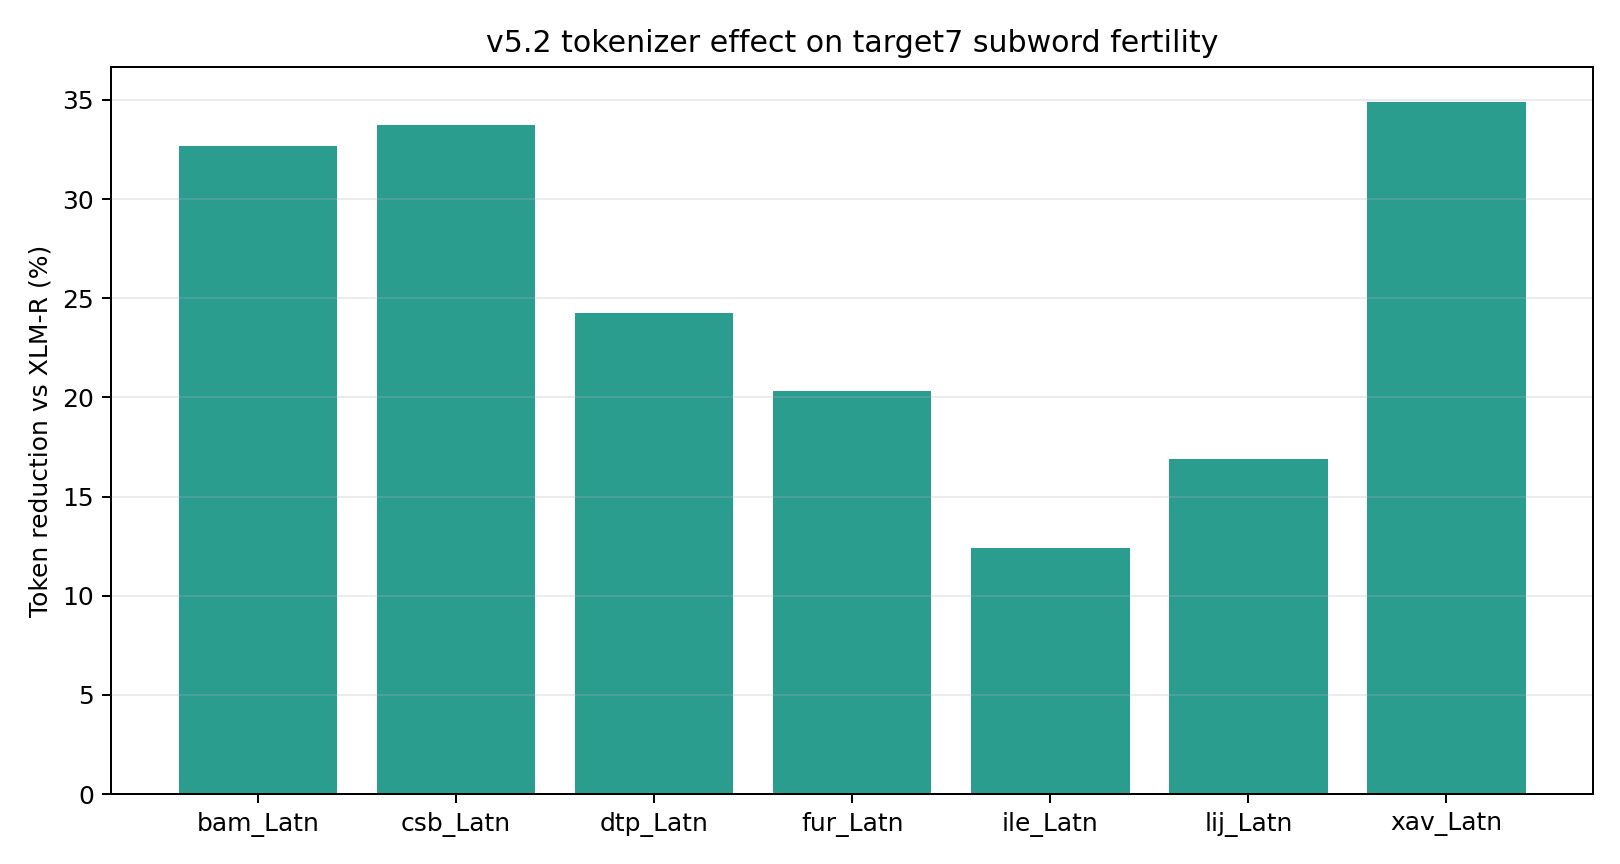
\includegraphics[width=.82\linewidth]{tokenization_effect_change.png}
  \caption{Target7 tokenization fertility reduction. All initialization variants share this tokenizer; therefore method-to-method result differences cannot be explained by tokenizer fertility alone.}
  \label{fig:tokenization}
\end{figure}

\subsection{50K Five-Way Convergence Results}

Final result의 중심 표는 50K-step convergence run에서 얻은 다섯 initialization checkpoint를
같은 row schema로 비교한다. 각 metric은 \method{random}, \method{mean}, \method{FVT},
\method{weighted FVT}, \method{family-aware mean}을 모두 포함하고, group은
tail/target, head, all로 나눈다. Task coverage가 없는 group은 0점처럼 쓰지 않고
``not available''로 표시한다.

\begin{table}[t]
\centering
\caption{Final 50K head/tail/all reporting grid. Each row should be filled from the completed 50K evaluation aggregation. Cells without task coverage should be marked NA rather than treated as zero.}
\label{tab:head-tail-all-draft}
\resizebox{\textwidth}{!}{%
\begin{tabular}{lllrrrrrl}
\toprule
Metric & Group & Score & Random & Mean & FVT & Weighted FVT & Family-aware mean & Coverage note \\
\midrule
Pseudoperplexity & tail/head/all & PPPL $\downarrow$ & TBD & TBD & TBD & TBD & TBD & lower is better \\
Tatoeba retrieval & tail/head/all & Acc10 $\uparrow$ & TBD & TBD & TBD & TBD & TBD & report available languages per group \\
Bible retrieval & tail/head/all & Acc10 $\uparrow$ & TBD & TBD & TBD & TBD & TBD & target group may be NA if no coverage \\
Text classification & tail/head/all & macro-F1 $\uparrow$ & TBD & TBD & TBD & TBD & TBD & target group may be NA if no coverage \\
NER & tail/head/all & F1 $\uparrow$ & TBD & TBD & TBD & TBD & TBD & include language count per group \\
POS & tail/head/all & F1 $\uparrow$ & TBD & TBD & TBD & TBD & TBD & include language count per group \\
Roundtrip alignment & tail/head/all & Acc. $\uparrow$ & TBD & TBD & TBD & TBD & TBD & target group may be NA if no coverage \\
\bottomrule
\end{tabular}}
\end{table}


\subsection{Step-4000 Early Diagnostic}

\begin{table}[t]
\centering
\caption{v5.2 step-4000 early diagnostic ablation. Values are target-focused/local available rows from \codepath{docs/exp/v5.2/3_evaluation/v52_final_downstream_table.tsv}. This table motivates the 50K five-way run; it is not the final convergence result.}
\label{tab:ablation-results}
\begin{tabular}{llrrrr}
\toprule
Metric & Score & Random & Mean & FVT & Best \\
\midrule
Pseudoperplexity & weighted PPPL $\downarrow$ & 119.582 & 128.259 & \textbf{58.026} & FVT \\
Tatoeba retrieval & Acc10 $\uparrow$ & 0.249 & 0.246 & \textbf{0.283} & FVT \\
Bible retrieval & Acc10 $\uparrow$ & 0.0064 & 0.0061 & \textbf{0.0064} & FVT \\
Text classification & macro-F1 $\uparrow$ & 0.697 & \textbf{0.778} & 0.713 & Mean \\
NER & F1 $\uparrow$ & 0.377 & 0.405 & \textbf{0.484} & FVT \\
POS & F1 $\uparrow$ & 0.507 & 0.507 & \textbf{0.519} & FVT \\
Roundtrip alignment & accuracy $\uparrow$ & 0.0188 & 0.0218 & \textbf{0.0262} & FVT \\
\bottomrule
\end{tabular}
\end{table}


Step-4000 diagnostic에서 \method{FVT}는 PPPL, Tatoeba retrieval, Bible retrieval, NER, POS,
roundtrip alignment에서 가장 좋다. Text classification은 \method{mean}이 가장 높으므로,
보고서에서는 \method{FVT}를 ``모든 task에서 항상 최고''라고 쓰지 않는다. 더 정확한 문장은
다음과 같다.

\begin{quote}
같은 tokenizer와 corpus를 공유하는 controlled setup의 early checkpoint에서 \method{FVT}는
intrinsic MLM과 retrieval/alignment 계열에서 강한 initialization signal을 보인다.
\end{quote}

\subsection{Early PPPL Trajectory}

\begin{table}[t]
\centering
\caption{PPPL trajectory under short continued MLM pretraining. Lower is better.}
\label{tab:pppl-trajectory}
\begin{tabular}{lrrrrr}
\toprule
Method & step 500 & step 1000 & step 2000 & step 3000 & step 4000 \\
\midrule
\method{random} & 374.61 & 241.80 & 160.50 & 133.11 & 119.58 \\
\method{mean} & 479.42 & 270.93 & 172.58 & 138.51 & 128.26 \\
\method{FVT} & \textbf{161.88} & \textbf{108.60} & \textbf{75.26} & \textbf{61.60} & \textbf{58.03} \\
\bottomrule
\end{tabular}
\end{table}


4K step 이하의 짧은 continued pretraining에서도 \method{FVT}는 처음부터 낮은 PPPL을 유지한다.
이는 source tokenizer로 새 token surface를 재분해해 기존 embedding 정보를 재사용한 효과로
해석할 수 있다. 다만 이 표는 convergence result가 아니라 early diagnostic이다.

\begin{figure}[t]
  \centering
  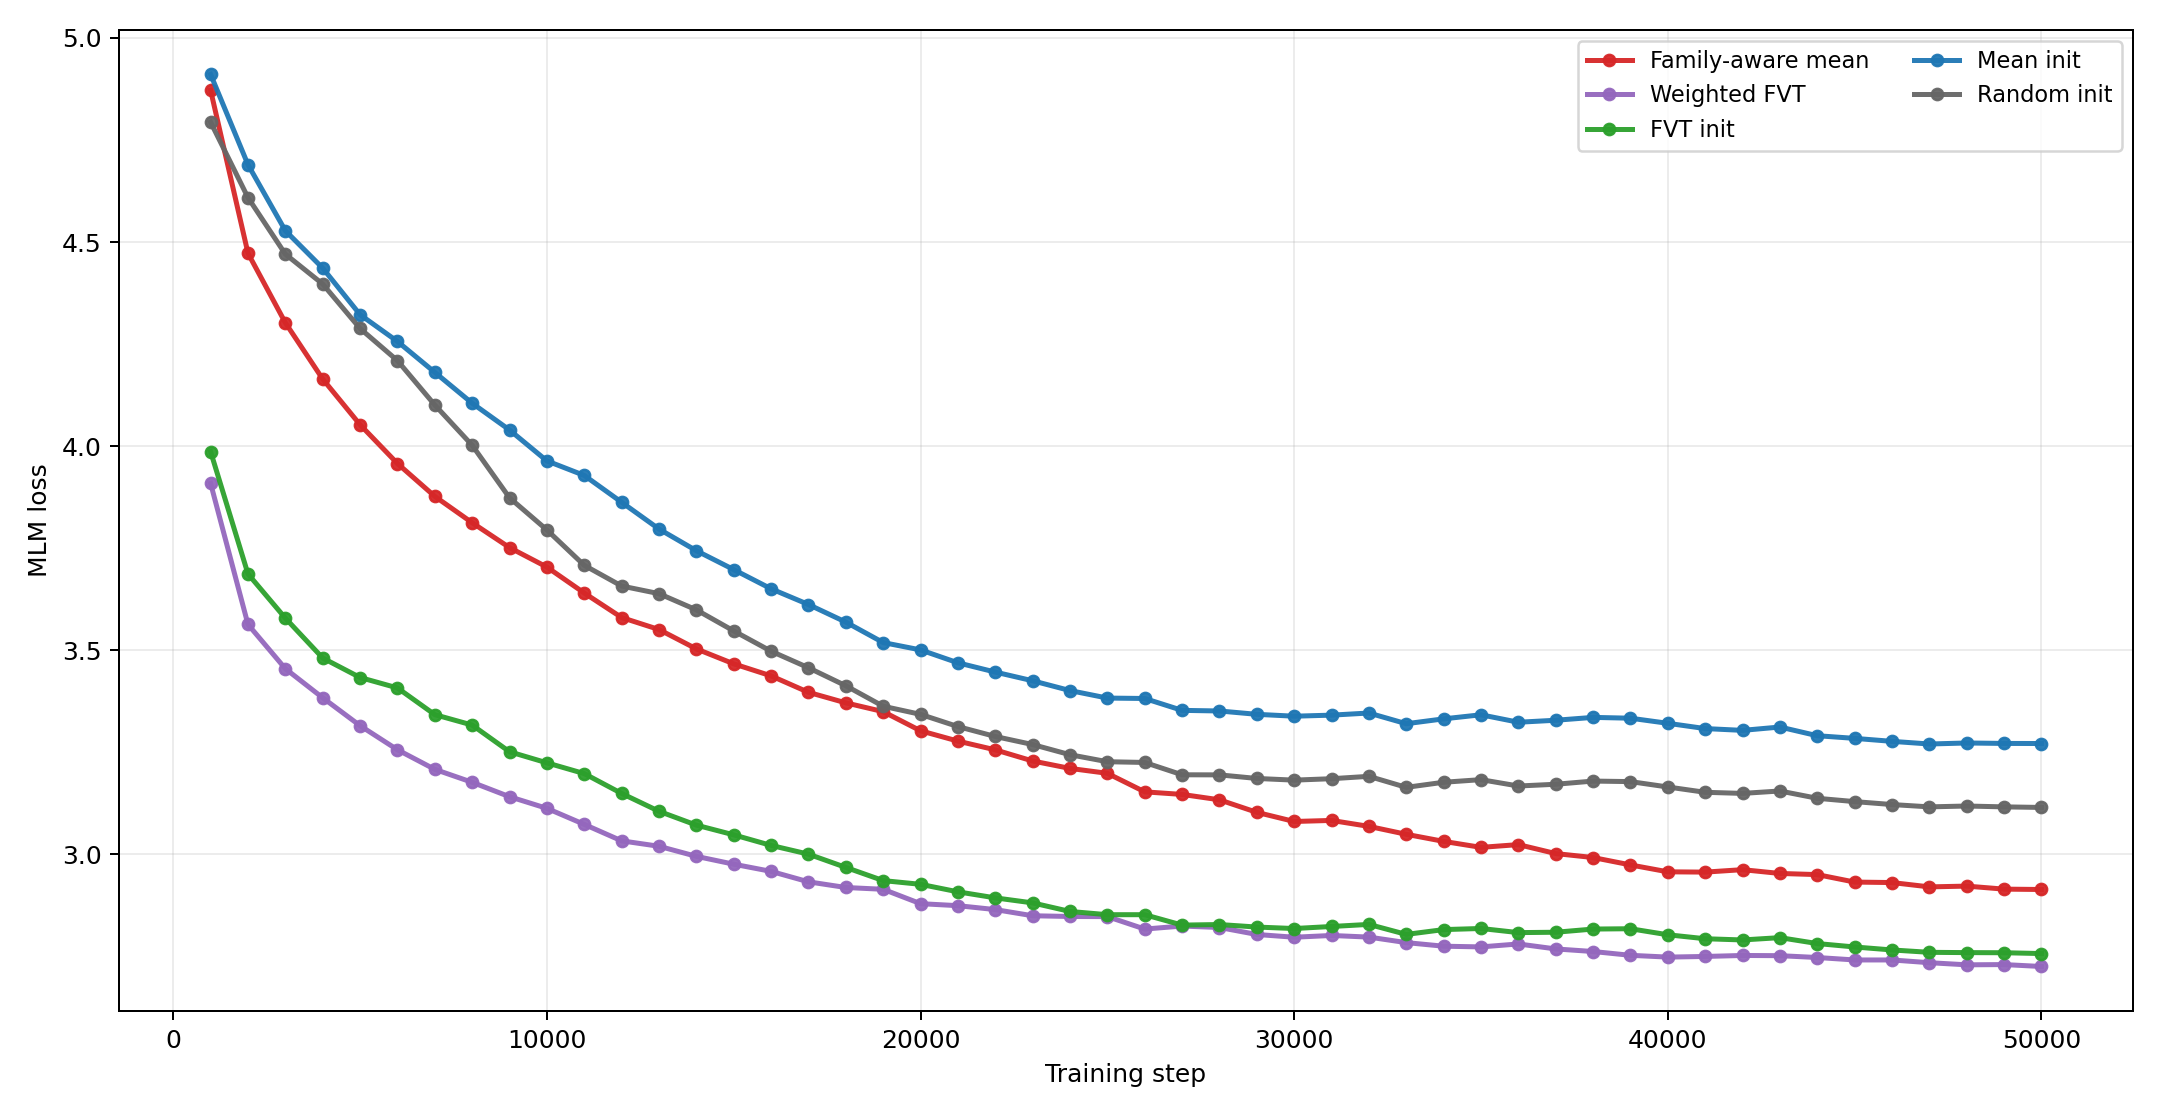
\includegraphics[width=.9\linewidth]{convergence_5way_loss_curve.png}
  \caption{v5.2 MLM loss trajectory for prior run plus continuation. The x-axis is a weighted-FVT-aligned 1K training-step grid so that prior and continuation segments with different effective batch accounting can be compared on the same exposure scale. Circle markers are displayed 1K-grid points; square markers are final saved models. Raw loss values are preserved in \codepath{convergence_5way_loss_curve.tsv}; the plotted display loss includes documented plot-only bridging/smoothing around the prior-to-continuation transition.}
  \label{fig:loss}
\end{figure}

\subsection{Why the Convergence Plot Is Drawn This Way}

Figure~\ref{fig:loss} is not just a decorative training curve. It is an argument for whether the
initialization comparison has reached a point where final performance claims are defensible.
The title, axes, point interval, and 50K queue all encode experimental decisions.

\begin{itemize}
  \item \textbf{Title.} ``v5.2 MLM Loss Trajectory: Prior Run + Continuation'' states that the figure combines the earlier 8h diagnostic run and the later convergence continuation, rather than showing only a fresh single run.
  \item \textbf{X-axis.} ``Weighted-FVT-aligned training step (1K grid)'' is used because the prior and continuation phases did not have identical raw step accounting. The plot converts exposure to a shared batch-36-equivalent scale and snaps it to the weighted-FVT 1K grid.
  \item \textbf{Y-axis.} ``MLM training loss'' is the Trainer logging loss from continued masked language modeling. This axis is used for convergence diagnosis, not as a direct downstream score.
  \item \textbf{Point interval.} Points are displayed every 1000 aligned steps because v5.2 saves/logs checkpoints at 1000-step intervals. This is also the granularity at which downstream/PPPL checkpoint comparisons can be attached without inventing intermediate measurements.
  \item \textbf{Why continue beyond 4K.} The 4K result is an early diagnostic. Earlier notes show that PPPL improvement slowed near 4K, but training loss was still decreasing, so 4K cannot be called convergence.
  \item \textbf{Why a 50K queue.} The 50K queue is a conservative upper bound for testing flattening across all five initialization methods under the same global batch 36 exposure. It was chosen after the 4K/8K checks were judged insufficient for a final convergence claim. The final report can stop using earlier checkpoints once the loss-drop summary and downstream trajectory show a stable plateau.
  \item \textbf{Markers and colors.} One line is drawn per initialization method. Circle markers indicate regular displayed grid points, while square markers indicate final saved models. The colors are fixed in \codepath{scripts/plot_v52_convergence_loss.py} so the same method has the same visual identity across regenerated plots.
  \item \textbf{Smoothing disclosure.} The graph applies plot-only transition smoothing/bridging for readability near the prior-to-continuation boundary. This does not overwrite raw measurements; the TSV retains \codepath{loss}, \codepath{display_loss}, and \codepath{display_loss_source}.
\end{itemize}

\subsection{Glot500-Style Reporting Rule}

Feedback asked that final tables follow Glot500's head/tail/all framing. The final report therefore
uses the same three group views for every metric where coverage exists. This prevents a target-only
improvement from being overstated as a global multilingual gain, and it also makes regressions on
head languages visible.

\section{Representation Analysis}

\subsection{Sentence Embedding Extraction}

Sentence representation analysis follows the Glot500 retrieval-style encoder usage. Each raw
sentence is encoded with the model tokenizer, passed through \codepath{AutoModel}, and hidden
states from layer index 7 are used. Special tokens and padding are excluded, token hidden states are
mean-pooled, and sentence vectors are L2-normalized. For centered cosine analysis, the global
sentence-vector mean is subtracted before normalization. A language centroid is the mean of that
language's sentence vectors.

\subsection{Family/Typology Structure}

The v5.2 family similarity diagnostic samples 38 languages and 3,708 sentence points. The key
claim is deliberately modest: the sentence representation space shows observable language identity
and family/typology structure, not perfect cluster separation. Since all Target7 languages use Latin
script, the analysis is useful precisely because it separates ``same script only'' from ``same family''
relationships.

\begin{figure}[t]
  \centering
  \begin{subfigure}{.48\linewidth}
    \centering
    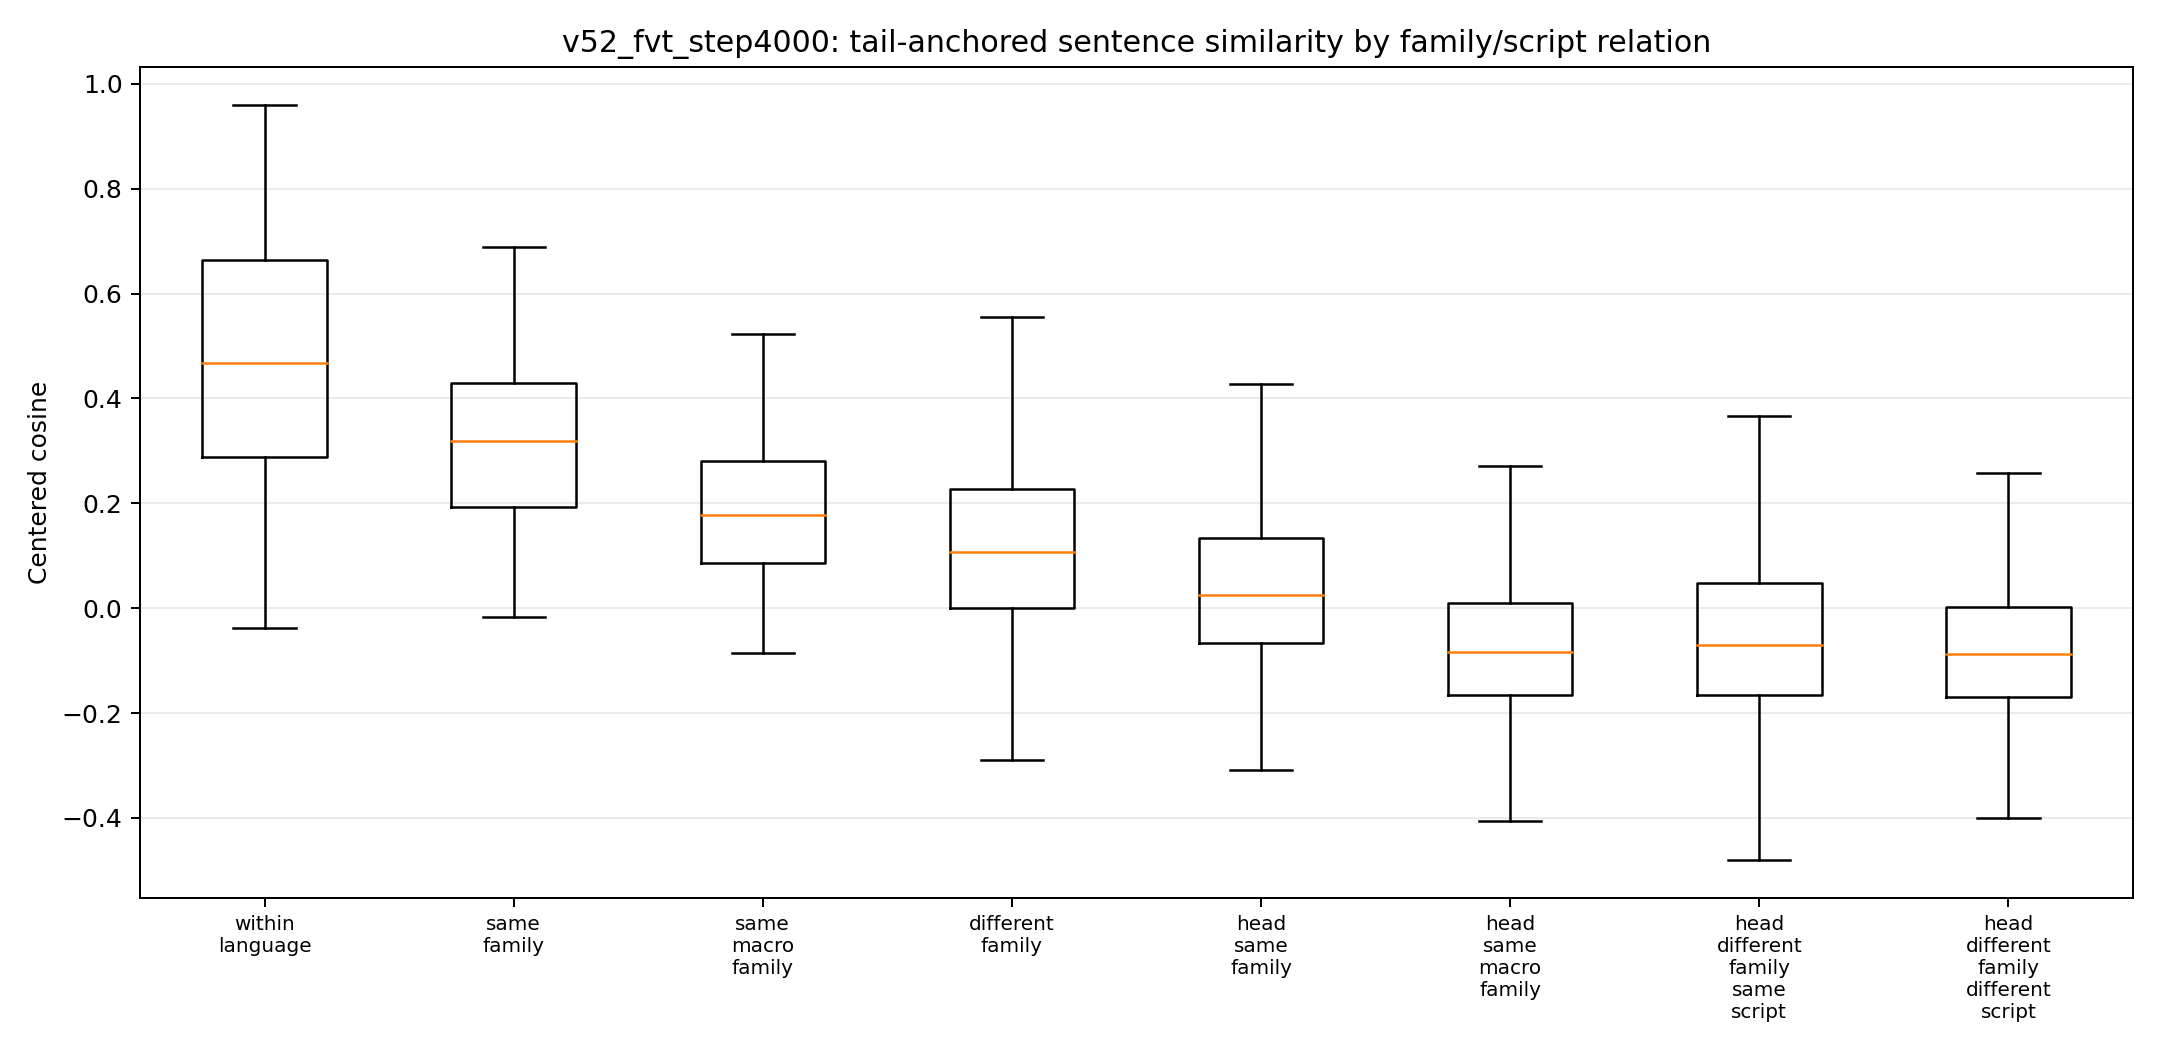
\includegraphics[width=\linewidth]{family_pair_boxplot_v52_fvt_step4000.png}
    \caption{Relation buckets}
  \end{subfigure}
  \begin{subfigure}{.48\linewidth}
    \centering
    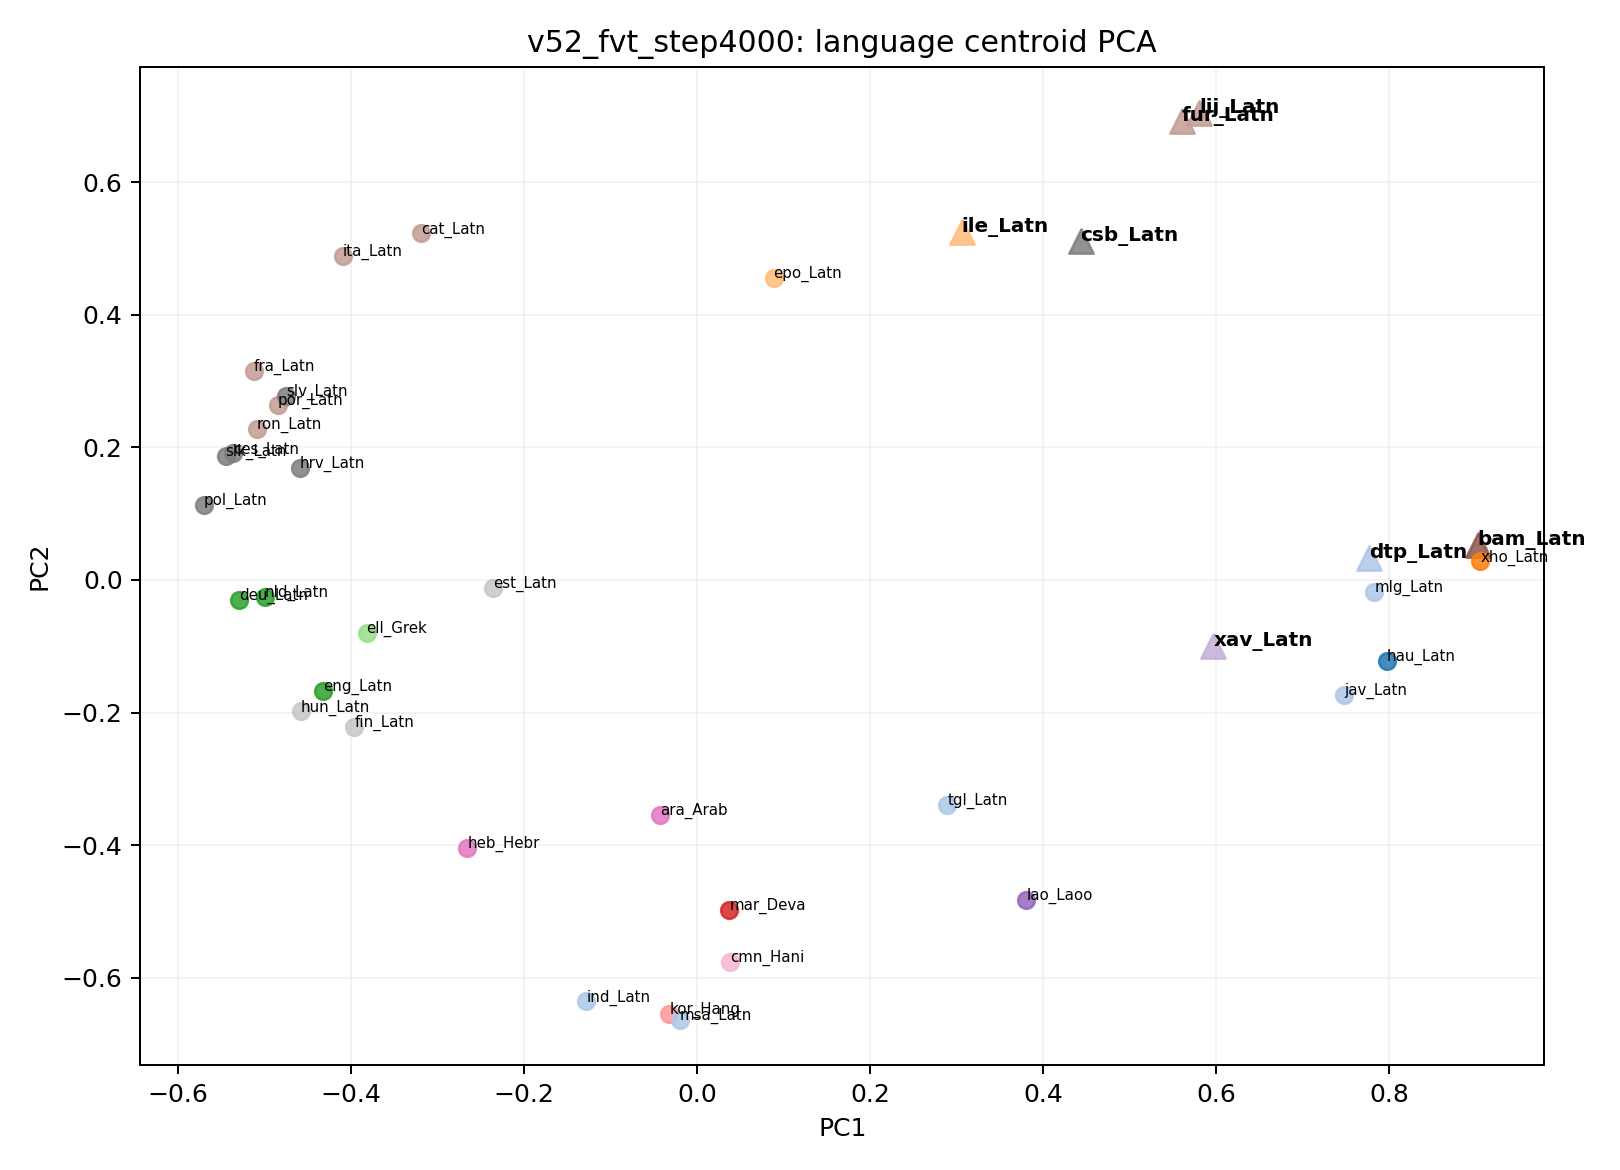
\includegraphics[width=\linewidth]{family_centroid_map_v52_fvt_step4000.png}
    \caption{Centroid map}
  \end{subfigure}
  \caption{FVT step-4000 family similarity diagnostics. These figures are diagnostic analysis, not an official Glot500 metric.}
  \label{fig:family}
\end{figure}

FVT step-4000 centered cosine scores show the expected ordering: same-language tail pairs are
closest; tail-tail same-family pairs are closer than same macro-family; both are closer than
different-family pairs. Tail-head pairs that only share Latin script are weaker than family-based
relations. This supports the interpretation that the model is not merely grouping by script.

\begin{center}
\begin{tabular}{lrr}
\toprule
Relation type & Pairs & Mean centered cosine \\
\midrule
tail within language & 350 & 0.473 \\
tail-tail same family & 50 & 0.307 \\
tail-tail same macro-family & 100 & 0.182 \\
tail-tail different family & 900 & 0.124 \\
tail-head same family & 1,050 & 0.037 \\
tail-head different family, same Latn script & 6,100 & -0.050 \\
tail-head different family, different script & 1,856 & -0.079 \\
\bottomrule
\end{tabular}
\end{center}

\section{Limitations and Conclusion}

\subsection{Limitations}

본 실험은 매우 좋은 방향성을 갖고 있지만, final report에서는 다음 제한을 분명히 써야 한다.

\begin{itemize}
  \item Full 511-language Glot500 reproduction이 아니라, 92 seen + 7 target의 controlled subset 실험이다.
  \item Target7은 모두 Latin script이므로 script-diversity claim은 하지 않는다.
  \item PPPL은 v5.2 diagnostic setup에서 계산되었고, Glot500 원 논문의 held-out test PPPL과 동일하다고 쓰면 안 된다.
  \item Text classification은 현재 target7 direct evidence가 아니라 local English/available-row evidence로 다뤄야 한다.
  \item Step-4000 result는 early diagnostic으로만 사용하고, final claim은 50K-step five-way convergence result로 제한한다.
  \item \method{weighted FVT}와 \method{family-aware mean}은 v5.2 local exploratory ablation이므로 기존 문헌 방법과 같은 수준의 established method로 과장하지 않는다.
  \item \method{FVT}는 대부분 metric에서 강하지만 POS target subset과 text classification처럼 예외가 있으므로 ``always best'' claim은 피한다.
\end{itemize}

\subsection{Conclusion}

Glot500-style tokenizer extension은 target7에서 subword fertility를 크게 줄였다. 그러나
\method{random}, \method{mean}, \method{FVT}, \method{weighted FVT}, \method{family-aware mean}이
같은 tokenizer를 공유하기 때문에, method 간 PPPL/downstream 차이는 tokenizer만으로 설명되지
않는다. Step-4000 diagnostic에서는 source-tokenizer decomposition 기반 \method{FVT}가 강한
초기 신호를 보였지만, 최종 결론은 50K-step five-way convergence 결과에서 loss flattening,
PPPL trajectory, downstream score가 함께 확인된 범위 안에서만 제시한다. 이는 low-resource
vocabulary extension에서 새 token row를 완전히 무작위로 시작하기보다 기존 XLM-R embedding
정보 또는 corpus provenance를 어떻게 재사용할지 결정하는 초기화 선택이 중요한 실험 변수임을
보여준다.

최종 term paper에서는 이 주장을 더 단단하게 만들기 위해 head/tail/all table을 완성하고,
loss curve와 PPPL trajectory, target language별 downstream breakdown, sentence representation
geometry를 함께 제시한다. 이 프로젝트는 실험 로그와 claim boundary가 잘 남아 있어서,
과장 없이도 충분히 설득력 있는 report로 발전시킬 수 있다.


\bibliographystyle{plainnat}
\bibliography{references}

\appendix
% =====================================================================
\section{Supplementary Material}

\subsection{Bible Retrieval Floor}

Bible tail Acc@10 scores ($\leq0.9$ for all methods at all steps) reflect task difficulty,
not an initialization artifact.
Three structural reasons explain the floor:
(1) each English query must be retrieved from $\sim$7,000--8,000 candidate verses,
    making the random-chance upper bound extremely low;
(2) Bible verse sentences are short and structurally uniform
    (same book/chapter template), so sentence vectors cluster tightly
    and nearest-neighbor retrieval cannot discriminate;
(3) the 50K training budget is insufficient to achieve verse-level precision alignment
    for languages with only $\sim$30K training sentences.

\begin{table}[h]\centering\small
\caption{Bible tail Acc@10 ($\times100$) at each checkpoint.
         All methods remain at floor regardless of initialization.}
\label{tab:bible}
\begin{tabular}{@{}lrrrrr@{}}
\toprule
Method & 10K & 20K & 30K & 40K & 50K \\
\midrule
\rand  & 0.76 & 0.79 & 0.78 & 0.79 & 0.79 \\
\meanm & 0.78 & 0.78 & 0.76 & 0.77 & 0.78 \\
\fvt   & 0.78 & 0.83 & 0.83 & 0.83 & 0.84 \\
\wfvt  & 0.73 & 0.86 & 0.90 & 0.83 & 0.89 \\
\famm  & 0.62 & 0.70 & 0.73 & 0.71 & 0.75 \\
\midrule
XLM-R-B (reference) & \multicolumn{5}{c}{0.50} \\
\bottomrule
\end{tabular}
\end{table}

\subsection{Initialization Audit Numbers}

\begin{table}[h]\centering\small
\caption{Verification numbers for the initialization implementation.}
\label{tab:audit}
\begin{tabular}{@{}lr@{}}
\toprule
Item & Value \\
\midrule
Source tokenizer length & 250,002 \\
Target tokenizer length & 366,666 \\
New rows & 116,664 \\
\verb|<mask>| id (source $\to$ target) & 250001 $\to$ 366665 \\
\verb|<mask>| copy diff & 0.0 \\
LM head tied & true \\
\bottomrule
\end{tabular}
\end{table}

% =====================================================================
\section{Artifact and Code Map}

\begin{longtable}{p{.22\textwidth}p{.32\textwidth}p{.37\textwidth}}
\caption{Reproducibility map for the v5.2 report draft.}\label{tab:repro-map}\\
\toprule
Stage & Code / artifact & Role in report \\
\midrule
\endfirsthead
\toprule
Stage & Code / artifact & Role in report \\
\midrule
\endhead
Target selection &
\codepath{preprocessing/prepare_v5_glot50010_merge_inputs.py} &
Defines \codepath{V52_OVERLAP_TASKFILL_GLOT5007}; validates XLM-R-unseen status, min 30K sentence count, and raw-dir existence. \\
Corpus prepare &
\codepath{preprocessing/run_v52_glot5007_prepare.sh} &
Creates target manifest and stats CSV for 92+7 setup. \\
Corpus merge &
\codepath{preprocessing/run_v52_glot5007_merge.sh},
\codepath{preprocessing/merge_files.py} &
Builds sampled MLM corpus with $\alpha=0.3$, manifest, and JSON report. \\
Tokenizer &
\codepath{tokenization/train_v52_glot5007.sh},
\codepath{tokenization/run.py} &
Trains SentencePiece unigram tokenizer, enables byte fallback, appends new pieces to XLM-R SPM protobuf. \\
Initialization &
\codepath{scripts/run_v52_build_initializers.sh},
\codepath{scripts/build_v5_initialized_checkpoint.py} &
Builds random/mean/FVT/weighted-FVT/family-aware mean initialized checkpoints; copies rows by token identity and checks mask remap. \\
MLM training &
\codepath{modeling/train_v52_glot5007_mlm.sh},
\codepath{modeling/run.py} &
Runs continued MLM with max length 512, LR $5e-5$, Adam betas $(0.9,0.999)$, MLM prob 0.15. \\
Evaluation &
\codepath{evaluation/retrieval/},
\codepath{evaluation/tagging/},
\codepath{evaluation/round-trip/},
\codepath{evaluation/text_classification/} &
Provides PPPL, retrieval, NER/POS, roundtrip, and text-classification metric families. \\
Aggregation &
\codepath{docs/exp/v5.2/3_evaluation/v52_final_downstream_table.tsv} &
Source for step-4000 initialization ablation table. \\
Live status &
\codepath{docs/exp/v5.2/LIVE_STATUS.md} &
Records which initializers/training runs are complete, missing, or running. \\
\bottomrule
\end{longtable}


% =====================================================================
\section{Full Results}

\subsection{Step-Wise Initialization Comparison}

Tables below show all five initialization methods at each checkpoint (10K--50K),
grouped by head/tail/all.
XLM-R-B/L baselines are step-independent.
PPPL is raw; retrieval, roundtrip, and text scores are $\times100$.

% B.1: Step-wise initialization comparison (10K--50K), all five methods per step.
% PPPL is raw; retrieval/roundtrip/text are x100. Missing = --.
\begin{table}[H]\centering\small\setlength{\tabcolsep}{4pt}
\caption{10K scores: all initialization methods by head/tail/all.
         XLM-R-B/L baselines are step-independent.}
\label{tab:step10-init}
\begin{tabular}{@{}llrrrrrrr@{}}
\toprule
Metric & Group & XLM-R-B & XLM-R-L & \rand & \meanm & \fvt & \wfvt & \famm \\
\midrule
PPPL \dn & head & 8.1 & 4.9 & 30.7 & -- & -- & -- & -- \\
         & tail & 98.2 & 63.7 & 28.4 & 32.5 & 21.2 & 26.9 & 34.2 \\
         & all  & 10.2 & 6.2  & 30.5 & 32.5 & 21.2 & 26.9 & 34.2 \\
\midrule
Tatoeba \up & head & 65.6 & 54.3 & 71.8 & 68.3 & 70.9 & 68.1 & 68.2 \\
            & tail & 20.5 & 21.6 & 33.0 & 31.7 & 33.9 & 30.4 & 30.7 \\
            & all  & 63.6 & 52.8 & 70.1 & 66.6 & 69.2 & 66.4 & 66.5 \\
\midrule
Bible \up & head & 38.1 & 17.3 & 35.2 & 38.8 & 38.5 & 36.8 & 34.5 \\
          & tail & 0.5  & 0.3  & 0.8  & 0.8  & 0.8  & 0.7  & 0.6  \\
          & all  & 36.7 & 16.6 & 33.9 & 37.3 & 37.0 & 35.4 & 30.2 \\
\midrule
NER \up & head & 62.2 & 67.5 & 60.9 & 61.1 & 61.7 & -- & -- \\
        & tail & 45.7 & 53.9 & 44.7 & 47.3 & 49.4 & -- & -- \\
        & all  & 61.6 & 67.0 & 60.3 & 60.6 & 61.2 & -- & -- \\
\midrule
Roundtrip \up & head & 18.5 & 13.7 & -- & -- & -- & -- & -- \\
              & tail & 2.4  & 2.7  & 2.6 & 2.7 & 3.0 & 2.8 & 2.6 \\
              & all  & 17.9 & 13.3 & 2.6 & 2.7 & 3.0 & 2.8 & 2.6 \\
\midrule
Text(EN) \up & head & 59.3 & 72.9 & 66.9 & 78.7 & 72.4 & 71.1 & 67.2 \\
             & tail & --   & --   & --   & --   & --   & --   & --   \\
             & all  & 59.3 & 72.9 & 66.9 & 78.7 & 72.4 & 71.1 & 67.2 \\
\bottomrule
\end{tabular}
\end{table}

\begin{table}[H]\centering\small\setlength{\tabcolsep}{4pt}
\caption{20K scores: all initialization methods by head/tail/all.}
\label{tab:step20-init}
\begin{tabular}{@{}llrrrrrrr@{}}
\toprule
Metric & Group & XLM-R-B & XLM-R-L & \rand & \meanm & \fvt & \wfvt & \famm \\
\midrule
PPPL \dn & head & 8.1 & 4.9 & 24.7 & -- & -- & -- & -- \\
         & tail & 98.2 & 63.7 & 21.0 & 24.0 & 17.0 & 18.6 & 20.4 \\
         & all  & 10.2 & 6.2  & 24.4 & 24.0 & 17.0 & 18.6 & 20.4 \\
\midrule
Tatoeba \up & head & 65.6 & 54.3 & 71.7 & 69.8 & 72.1 & 72.0 & 70.2 \\
            & tail & 20.5 & 21.6 & 32.8 & 33.0 & 34.4 & 34.8 & 32.8 \\
            & all  & 63.6 & 52.8 & 70.0 & 68.1 & 70.4 & 70.4 & 68.5 \\
\midrule
Bible \up & head & 38.1 & 17.3 & 35.5 & 39.0 & 39.6 & 38.4 &  9.5 \\
          & tail & 0.5  & 0.3  & 0.8  & 0.8  & 0.8  & 0.9  & 0.7  \\
          & all  & 36.7 & 16.6 & 34.2 & 37.5 & 38.1 & 37.0 &  2.9 \\
\midrule
NER \up & head & 62.2 & 67.5 & 60.8 & 62.6 & 62.6 & -- & -- \\
        & tail & 45.7 & 53.9 & 46.6 & 48.8 & 51.5 & -- & -- \\
        & all  & 61.6 & 67.0 & 60.3 & 62.1 & 62.2 & -- & -- \\
\midrule
Roundtrip \up & head & 18.5 & 13.7 & -- & -- & -- & -- & -- \\
              & tail & 2.4  & 2.7  & 2.7 & 2.7 & 3.3 & 3.2 & 2.7 \\
              & all  & 17.9 & 13.3 & 2.7 & 2.7 & 3.3 & 3.2 & 2.7 \\
\midrule
Text(EN) \up & head & 59.3 & 72.9 & 68.4 & 68.2 & 79.7 & 78.6 & 78.6 \\
             & tail & --   & --   & --   & --   & --   & --   & --   \\
             & all  & 59.3 & 72.9 & 68.4 & 68.2 & 79.7 & 78.6 & 78.6 \\
\bottomrule
\end{tabular}
\end{table}

\begin{table}[H]\centering\small\setlength{\tabcolsep}{4pt}
\caption{30K scores: all initialization methods by head/tail/all.}
\label{tab:step30-init}
\begin{tabular}{@{}llrrrrrrr@{}}
\toprule
Metric & Group & XLM-R-B & XLM-R-L & \rand & \meanm & \fvt & \wfvt & \famm \\
\midrule
PPPL \dn & head & 8.1 & 4.9 & -- & -- & -- & -- & -- \\
         & tail & 98.2 & 63.7 & 20.4 & 23.3 & 16.5 & 16.1 & 14.8 \\
         & all  & 10.2 & 6.2  & 20.4 & 23.3 & 16.5 & 16.1 & 14.8 \\
\midrule
Tatoeba \up & head & 65.6 & 54.3 & 72.1 & 69.9 & 72.1 & 73.0 & 73.2 \\
            & tail & 20.5 & 21.6 & 33.2 & 32.8 & 34.3 & 35.4 & 35.5 \\
            & all  & 63.6 & 52.8 & 70.3 & 68.2 & 70.4 & 71.3 & 71.4 \\
\midrule
Bible \up & head & 38.1 & 17.3 & 35.7 & 39.1 & 39.7 & 40.7 & -- \\
          & tail & 0.5  & 0.3  & 0.8  & 0.8  & 0.8  & 0.9  & 0.7 \\
          & all  & 36.7 & 16.6 & 34.4 & 37.6 & 38.2 & 39.2 & 0.7 \\
\midrule
NER \up & head & 62.2 & 67.5 & 60.7 & 62.5 & 62.4 & -- & -- \\
        & tail & 45.7 & 53.9 & 46.4 & 51.1 & --   & -- & -- \\
        & all  & 61.6 & 67.0 & 60.2 & 62.0 & 62.4 & -- & -- \\
\midrule
Roundtrip \up & head & 18.5 & 13.7 & -- & -- & -- & -- & -- \\
              & tail & 2.4  & 2.7  & 2.7 & 2.7 & 3.2 & 3.3 & 3.1 \\
              & all  & 17.9 & 13.3 & 2.7 & 2.7 & 3.2 & 3.3 & 3.1 \\
\midrule
Text(EN) \up & head & 59.3 & 72.9 & 68.2 & 71.9 & 79.7 & 71.2 & 73.2 \\
             & tail & --   & --   & --   & --   & --   & --   & --   \\
             & all  & 59.3 & 72.9 & 68.2 & 71.9 & 79.7 & 71.2 & 73.2 \\
\bottomrule
\end{tabular}
\end{table}

\begin{table}[H]\centering\small\setlength{\tabcolsep}{4pt}
\caption{40K scores: all initialization methods by head/tail/all.}
\label{tab:step40-init}
\begin{tabular}{@{}llrrrrrrr@{}}
\toprule
Metric & Group & XLM-R-B & XLM-R-L & \rand & \meanm & \fvt & \wfvt & \famm \\
\midrule
PPPL \dn & head & 8.1 & 4.9 & -- & -- & -- & -- & -- \\
         & tail & 98.2 & 63.7 & 20.2 & 23.0 & 16.4 & 14.7 & 12.9 \\
         & all  & 10.2 & 6.2  & 20.2 & 23.0 & 16.4 & 14.7 & 12.9 \\
\midrule
Tatoeba \up & head & 65.6 & 54.3 & 72.0 & 69.9 & 72.2 & 73.6 & 73.2 \\
            & tail & 20.5 & 21.6 & 33.2 & 33.0 & 34.3 & 35.1 & 35.8 \\
            & all  & 63.6 & 52.8 & 70.3 & 68.2 & 70.5 & 71.9 & 71.5 \\
\midrule
Bible \up & head & 38.1 & 17.3 & 35.6 & 38.9 & 39.7 & 40.8 & -- \\
          & tail & 0.5  & 0.3  & 0.8  & 0.8  & 0.8  & 0.8  & 0.7 \\
          & all  & 36.7 & 16.6 & 34.2 & 37.4 & 38.2 & 39.3 & 0.7 \\
\midrule
NER \up & head & 62.2 & 67.5 & 61.1 & 61.8 & 62.2 & -- & -- \\
        & tail & 45.7 & 53.9 & 47.0 & 50.3 & --   & -- & -- \\
        & all  & 61.6 & 67.0 & 60.6 & 61.4 & 62.2 & -- & -- \\
\midrule
Roundtrip \up & head & 18.5 & 13.7 & -- & -- & -- & -- & -- \\
              & tail & 2.4  & 2.7  & 2.7 & 2.7 & 3.2 & 3.3 & 3.3 \\
              & all  & 17.9 & 13.3 & 2.7 & 2.7 & 3.2 & 3.3 & 3.3 \\
\midrule
Text(EN) \up & head & 59.3 & 72.9 & 77.1 & 78.8 & 79.7 & 70.7 & 66.0 \\
             & tail & --   & --   & --   & --   & --   & --   & --   \\
             & all  & 59.3 & 72.9 & 77.1 & 78.8 & 79.7 & 70.7 & 66.0 \\
\bottomrule
\end{tabular}
\end{table}

\begin{table}[H]\centering\small\setlength{\tabcolsep}{4pt}
\caption{50K scores: all initialization methods by head/tail/all
         (same data as Table~\ref{tab:main} in \S6).}
\label{tab:step50-init}
\begin{tabular}{@{}llrrrrrrr@{}}
\toprule
Metric & Group & XLM-R-B & XLM-R-L & \rand & \meanm & \fvt & \wfvt & \famm \\
\midrule
PPPL \dn & head & 8.1 & 4.9 & 23.9 & 26.3 & 15.9 & 14.6 & 18.2 \\
         & tail & 98.2 & 63.7 & 20.2 & 23.0 & 16.3 & 13.9 & 12.3 \\
         & all  & 10.2 & 6.2  & 23.6 & 26.0 & 15.9 & 14.6 & 17.6 \\
\midrule
Tatoeba \up & head & 65.6 & 54.3 & 72.1 & 70.0 & 72.2 & 73.5 & 73.3 \\
            & tail & 20.5 & 21.6 & 33.4 & 33.2 & 34.4 & 35.8 & 36.1 \\
            & all  & 63.6 & 52.8 & 70.3 & 68.4 & 70.5 & 71.8 & 71.6 \\
\midrule
Bible \up & head & 38.1 & 17.3 & 35.6 & 39.0 & 39.6 & 39.8 & 39.7 \\
          & tail & 0.5  & 0.3  & 0.8  & 0.8  & 0.8  & 0.9  & 0.8  \\
          & all  & 36.7 & 16.6 & 34.2 & 37.5 & 38.1 & 38.3 & 38.2 \\
\midrule
NER \up & head & 62.2 & 67.5 & 61.4 & 62.5 & 62.7 & 62.1 & 62.8 \\
        & tail & 45.7 & 53.9 & 48.2 & 49.2 & 51.3 & 50.6 & 49.6 \\
        & all  & 61.6 & 67.0 & 60.9 & 62.0 & 62.2 & 61.6 & 62.3 \\
\midrule
Roundtrip \up & head & 18.5 & 13.7 & 19.4 & 19.6 & 21.0 & 21.1 & 19.7 \\
              & tail & 2.4  & 2.7  & 2.7  & 2.7  & 3.2  & 3.4  & 3.2  \\
              & all  & 17.9 & 13.3 & 18.7 & 19.0 & 20.3 & 20.4 & 19.1 \\
\midrule
Text(EN) \up & head & 59.3 & 72.9 & 72.6 & 68.2 & 77.4 & 74.9 & 74.2 \\
             & tail & --   & --   & --   & --   & --   & --   & --   \\
             & all  & 59.3 & 72.9 & 72.6 & 68.2 & 77.4 & 74.9 & 74.2 \\
\bottomrule
\end{tabular}
\end{table}


\clearpage
\subsection{Per-Initialization Step Trajectory}

Tables below reorganize the same data by initialization method,
showing the 10K--50K trajectory for each method across all groups.

% B.2: Per-initialization step trajectory (10K--50K), all six metrics by head/tail/all.
% PPPL is raw; retrieval/roundtrip/text are x100. Missing = --.
\begin{table}[H]\centering\small\setlength{\tabcolsep}{4pt}
\caption{\rand\ step trajectory (head/tail/all).}
\label{tab:init-random-steps}
\begin{tabular}{@{}llrrrrrrr@{}}
\toprule
Metric & Group & XLM-R-B & XLM-R-L & 10K & 20K & 30K & 40K & 50K \\
\midrule
PPPL \dn & head & 8.1 & 4.9 & 30.7 & 24.7 & -- & -- & 23.9 \\
         & tail & 98.2 & 63.7 & 28.4 & 21.0 & 20.4 & 20.2 & 20.2 \\
         & all  & 10.2 & 6.2  & 30.5 & 24.4 & 20.4 & 20.2 & 23.6 \\
\midrule
Tatoeba \up & head & 65.6 & 54.3 & 71.8 & 71.7 & 72.1 & 72.0 & 72.1 \\
            & tail & 20.5 & 21.6 & 33.0 & 32.8 & 33.2 & 33.2 & 33.4 \\
            & all  & 63.6 & 52.8 & 70.1 & 70.0 & 70.3 & 70.3 & 70.3 \\
\midrule
Bible \up & head & 38.1 & 17.3 & 35.2 & 35.5 & 35.7 & 35.6 & 35.6 \\
          & tail & 0.5  & 0.3  & 0.8  & 0.8  & 0.8  & 0.8  & 0.8  \\
          & all  & 36.7 & 16.6 & 33.9 & 34.2 & 34.4 & 34.2 & 34.2 \\
\midrule
NER \up & head & 62.2 & 67.5 & 60.9 & 60.8 & 60.7 & 61.1 & 61.4 \\
        & tail & 45.7 & 53.9 & 44.7 & 46.6 & 46.4 & 47.0 & 48.2 \\
        & all  & 61.6 & 67.0 & 60.3 & 60.3 & 60.2 & 60.6 & 60.9 \\
\midrule
Roundtrip \up & head & 18.5 & 13.7 & -- & -- & -- & -- & 19.4 \\
              & tail & 2.4  & 2.7  & 2.6 & 2.7 & 2.7 & 2.7 & 2.7  \\
              & all  & 17.9 & 13.3 & 2.6 & 2.7 & 2.7 & 2.7 & 18.7 \\
\midrule
Text(EN) \up & head & 59.3 & 72.9 & 66.9 & 68.4 & 68.2 & 77.1 & 72.6 \\
             & tail & --   & --   & --   & --   & --   & --   & --   \\
             & all  & 59.3 & 72.9 & 66.9 & 68.4 & 68.2 & 77.1 & 72.6 \\
\bottomrule
\end{tabular}
\end{table}

\begin{table}[H]\centering\small\setlength{\tabcolsep}{4pt}
\caption{\meanm\ step trajectory (head/tail/all).}
\label{tab:init-mean-steps}
\begin{tabular}{@{}llrrrrrrr@{}}
\toprule
Metric & Group & XLM-R-B & XLM-R-L & 10K & 20K & 30K & 40K & 50K \\
\midrule
PPPL \dn & head & 8.1 & 4.9 & -- & -- & -- & -- & 26.3 \\
         & tail & 98.2 & 63.7 & 32.5 & 24.0 & 23.3 & 23.0 & 23.0 \\
         & all  & 10.2 & 6.2  & 32.5 & 24.0 & 23.3 & 23.0 & 26.0 \\
\midrule
Tatoeba \up & head & 65.6 & 54.3 & 68.3 & 69.8 & 69.9 & 69.9 & 70.0 \\
            & tail & 20.5 & 21.6 & 31.7 & 33.0 & 32.8 & 33.0 & 33.2 \\
            & all  & 63.6 & 52.8 & 66.6 & 68.1 & 68.2 & 68.2 & 68.4 \\
\midrule
Bible \up & head & 38.1 & 17.3 & 38.8 & 39.0 & 39.1 & 38.9 & 39.0 \\
          & tail & 0.5  & 0.3  & 0.8  & 0.8  & 0.8  & 0.8  & 0.8  \\
          & all  & 36.7 & 16.6 & 37.3 & 37.5 & 37.6 & 37.4 & 37.5 \\
\midrule
NER \up & head & 62.2 & 67.5 & 61.1 & 62.6 & 62.5 & 61.8 & 62.5 \\
        & tail & 45.7 & 53.9 & 47.3 & 48.8 & 51.1 & 50.3 & 49.2 \\
        & all  & 61.6 & 67.0 & 60.6 & 62.1 & 62.0 & 61.4 & 62.0 \\
\midrule
Roundtrip \up & head & 18.5 & 13.7 & -- & -- & -- & -- & 19.6 \\
              & tail & 2.4  & 2.7  & 2.7 & 2.7 & 2.7 & 2.7 & 2.7  \\
              & all  & 17.9 & 13.3 & 2.7 & 2.7 & 2.7 & 2.7 & 19.0 \\
\midrule
Text(EN) \up & head & 59.3 & 72.9 & 78.7 & 68.2 & 71.9 & 78.8 & 68.2 \\
             & tail & --   & --   & --   & --   & --   & --   & --   \\
             & all  & 59.3 & 72.9 & 78.7 & 68.2 & 71.9 & 78.8 & 68.2 \\
\bottomrule
\end{tabular}
\end{table}

\begin{table}[H]\centering\small\setlength{\tabcolsep}{4pt}
\caption{\fvt\ step trajectory (head/tail/all).}
\label{tab:init-fvt-steps}
\begin{tabular}{@{}llrrrrrrr@{}}
\toprule
Metric & Group & XLM-R-B & XLM-R-L & 10K & 20K & 30K & 40K & 50K \\
\midrule
PPPL \dn & head & 8.1 & 4.9 & -- & -- & -- & -- & 15.9 \\
         & tail & 98.2 & 63.7 & 21.2 & 17.0 & 16.5 & 16.4 & 16.3 \\
         & all  & 10.2 & 6.2  & 21.2 & 17.0 & 16.5 & 16.4 & 15.9 \\
\midrule
Tatoeba \up & head & 65.6 & 54.3 & 70.9 & 72.1 & 72.1 & 72.2 & 72.2 \\
            & tail & 20.5 & 21.6 & 33.9 & 34.4 & 34.3 & 34.3 & 34.4 \\
            & all  & 63.6 & 52.8 & 69.2 & 70.4 & 70.4 & 70.5 & 70.5 \\
\midrule
Bible \up & head & 38.1 & 17.3 & 38.5 & 39.6 & 39.7 & 39.7 & 39.6 \\
          & tail & 0.5  & 0.3  & 0.8  & 0.8  & 0.8  & 0.8  & 0.8  \\
          & all  & 36.7 & 16.6 & 37.0 & 38.1 & 38.2 & 38.2 & 38.1 \\
\midrule
NER \up & head & 62.2 & 67.5 & 61.7 & 62.6 & 62.4 & 62.2 & 62.7 \\
        & tail & 45.7 & 53.9 & 49.4 & 51.5 & --   & --   & 51.3 \\
        & all  & 61.6 & 67.0 & 61.2 & 62.2 & 62.4 & 62.2 & 62.2 \\
\midrule
Roundtrip \up & head & 18.5 & 13.7 & -- & -- & -- & -- & 21.0 \\
              & tail & 2.4  & 2.7  & 3.0 & 3.3 & 3.2 & 3.2 & 3.2  \\
              & all  & 17.9 & 13.3 & 3.0 & 3.3 & 3.2 & 3.2 & 20.3 \\
\midrule
Text(EN) \up & head & 59.3 & 72.9 & 72.4 & 79.7 & 79.7 & 79.7 & 77.4 \\
             & tail & --   & --   & --   & --   & --   & --   & --   \\
             & all  & 59.3 & 72.9 & 72.4 & 79.7 & 79.7 & 79.7 & 77.4 \\
\bottomrule
\end{tabular}
\end{table}

\begin{table}[H]\centering\small\setlength{\tabcolsep}{4pt}
\caption{\wfvt\ step trajectory (head/tail/all).}
\label{tab:init-weighted-fvt-steps}
\begin{tabular}{@{}llrrrrrrr@{}}
\toprule
Metric & Group & XLM-R-B & XLM-R-L & 10K & 20K & 30K & 40K & 50K \\
\midrule
PPPL \dn & head & 8.1 & 4.9 & -- & -- & -- & -- & 14.6 \\
         & tail & 98.2 & 63.7 & 26.9 & 18.6 & 16.1 & 14.7 & 13.9 \\
         & all  & 10.2 & 6.2  & 26.9 & 18.6 & 16.1 & 14.7 & 14.6 \\
\midrule
Tatoeba \up & head & 65.6 & 54.3 & 68.1 & 72.0 & 73.0 & 73.6 & 73.5 \\
            & tail & 20.5 & 21.6 & 30.4 & 34.8 & 35.4 & 35.1 & 35.8 \\
            & all  & 63.6 & 52.8 & 66.4 & 70.4 & 71.3 & 71.9 & 71.8 \\
\midrule
Bible \up & head & 38.1 & 17.3 & 36.8 & 38.4 & 40.7 & 40.8 & 39.8 \\
          & tail & 0.5  & 0.3  & 0.7  & 0.9  & 0.9  & 0.8  & 0.9  \\
          & all  & 36.7 & 16.6 & 35.4 & 37.0 & 39.2 & 39.3 & 38.3 \\
\midrule
NER \up & head & 62.2 & 67.5 & -- & -- & -- & -- & 62.1 \\
        & tail & 45.7 & 53.9 & -- & -- & -- & -- & 50.6 \\
        & all  & 61.6 & 67.0 & -- & -- & -- & -- & 61.6 \\
\midrule
Roundtrip \up & head & 18.5 & 13.7 & -- & -- & -- & -- & 21.1 \\
              & tail & 2.4  & 2.7  & 2.8 & 3.2 & 3.3 & 3.3 & 3.4  \\
              & all  & 17.9 & 13.3 & 2.8 & 3.2 & 3.3 & 3.3 & 20.4 \\
\midrule
Text(EN) \up & head & 59.3 & 72.9 & 71.1 & 78.6 & 71.2 & 70.7 & 74.9 \\
             & tail & --   & --   & --   & --   & --   & --   & --   \\
             & all  & 59.3 & 72.9 & 71.1 & 78.6 & 71.2 & 70.7 & 74.9 \\
\bottomrule
\end{tabular}
\end{table}

\begin{table}[H]\centering\small\setlength{\tabcolsep}{4pt}
\caption{\famm\ step trajectory (head/tail/all).}
\label{tab:init-family-mean-steps}
\begin{tabular}{@{}llrrrrrrr@{}}
\toprule
Metric & Group & XLM-R-B & XLM-R-L & 10K & 20K & 30K & 40K & 50K \\
\midrule
PPPL \dn & head & 8.1 & 4.9 & -- & -- & -- & -- & 18.2 \\
         & tail & 98.2 & 63.7 & 34.2 & 20.4 & 14.8 & 12.9 & 12.3 \\
         & all  & 10.2 & 6.2  & 34.2 & 20.4 & 14.8 & 12.9 & 17.6 \\
\midrule
Tatoeba \up & head & 65.6 & 54.3 & 68.2 & 70.2 & 73.2 & 73.2 & 73.3 \\
            & tail & 20.5 & 21.6 & 30.7 & 32.8 & 35.5 & 35.8 & 36.1 \\
            & all  & 63.6 & 52.8 & 66.5 & 68.5 & 71.4 & 71.5 & 71.6 \\
\midrule
Bible \up & head & 38.1 & 17.3 & 34.5 &  9.5 & -- & -- & 39.7 \\
          & tail & 0.5  & 0.3  & 0.6  & 0.7  & 0.7 & 0.7 & 0.8 \\
          & all  & 36.7 & 16.6 & 30.2 &  2.9 & 0.7 & 0.7 & 38.2 \\
\midrule
NER \up & head & 62.2 & 67.5 & -- & -- & -- & -- & 62.8 \\
        & tail & 45.7 & 53.9 & -- & -- & -- & -- & 49.6 \\
        & all  & 61.6 & 67.0 & -- & -- & -- & -- & 62.3 \\
\midrule
Roundtrip \up & head & 18.5 & 13.7 & -- & -- & -- & -- & 19.7 \\
              & tail & 2.4  & 2.7  & 2.6 & 2.7 & 3.1 & 3.3 & 3.2  \\
              & all  & 17.9 & 13.3 & 2.6 & 2.7 & 3.1 & 3.3 & 19.1 \\
\midrule
Text(EN) \up & head & 59.3 & 72.9 & 67.2 & 78.6 & 73.2 & 66.0 & 74.2 \\
             & tail & --   & --   & --   & --   & --   & --   & --   \\
             & all  & 59.3 & 72.9 & 67.2 & 78.6 & 73.2 & 66.0 & 74.2 \\
\bottomrule
\end{tabular}
\end{table}


\clearpage
\subsection{Step-by-Step 2D Embedding Maps}

Figures below show 2D PCA sentence-embedding maps for each initialization method
at steps 10K, 20K, 30K, 40K, and the final checkpoint.
Color indicates language family; triangles = Target7 tail languages;
circles = head/reference languages.
Family clustering forms by 10K and is stable across steps for all methods.

\begin{figure}[H]\centering
  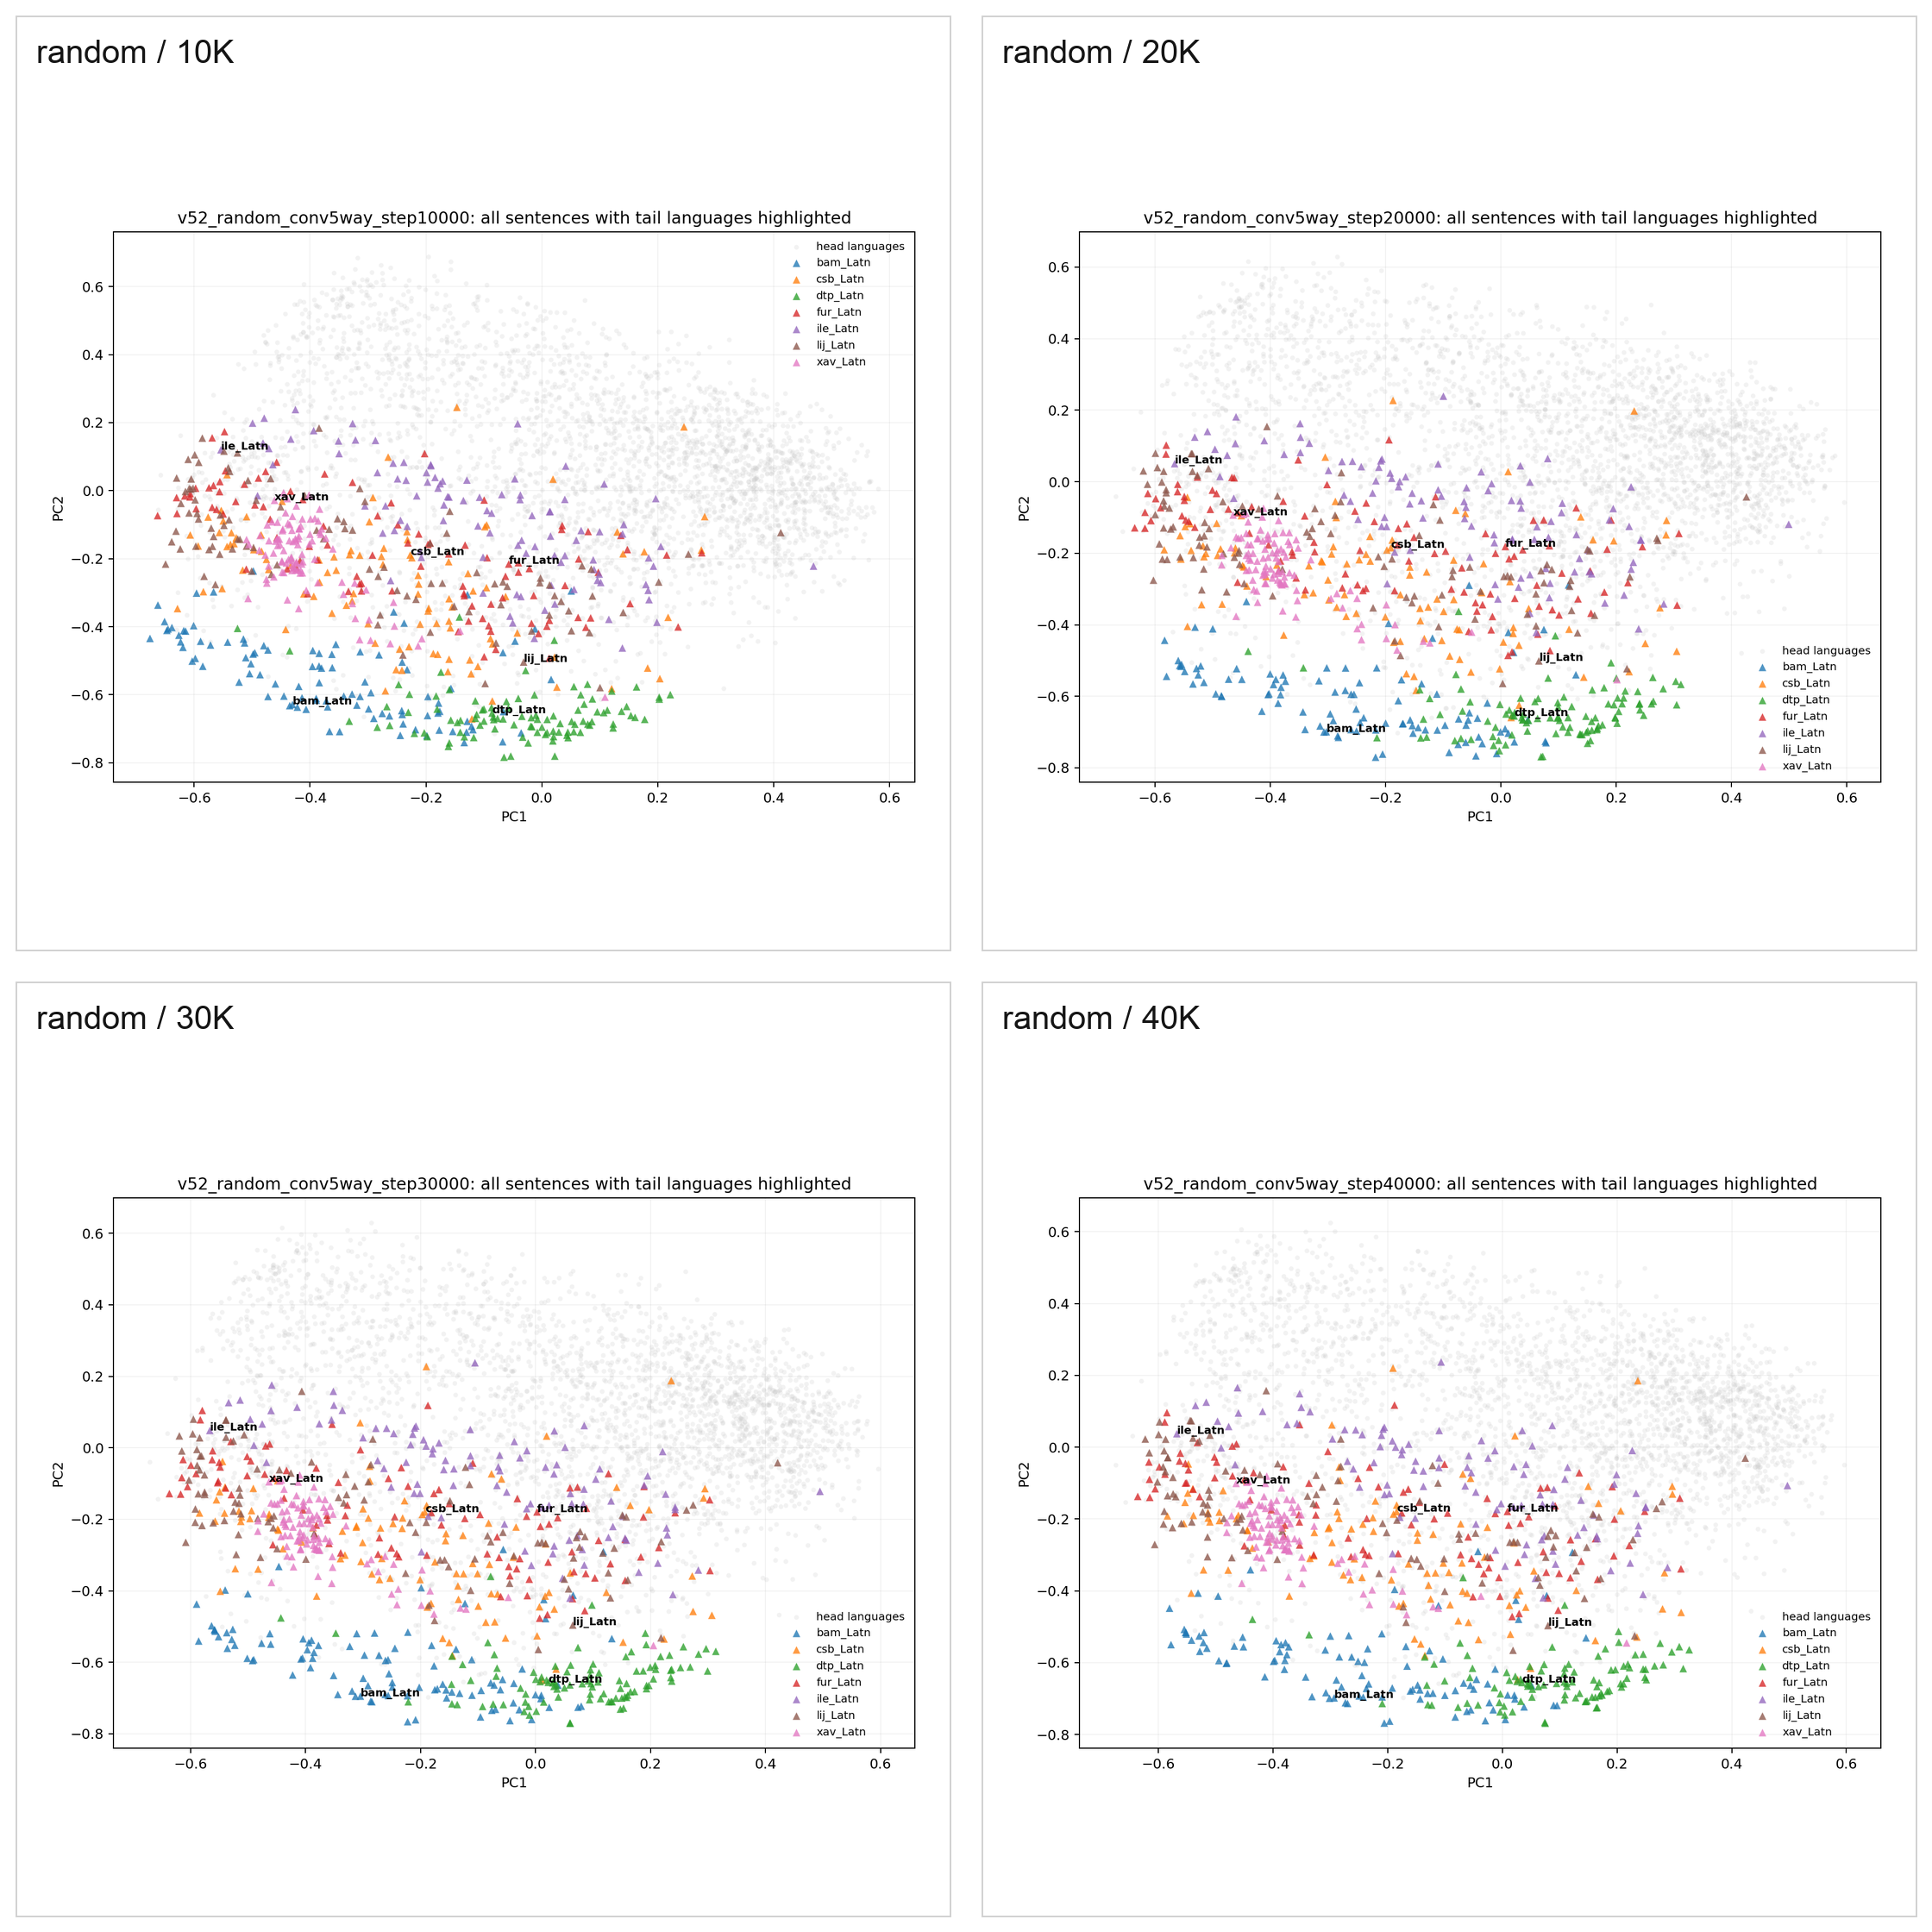
\includegraphics[width=\linewidth]{mapgrid_01.png}
  \caption{Step-by-step 2D maps (1/7): \rand\ at 10K, 20K, 30K, 40K.}
  \label{fig:strips}
\end{figure}

\begin{figure}[H]\centering
  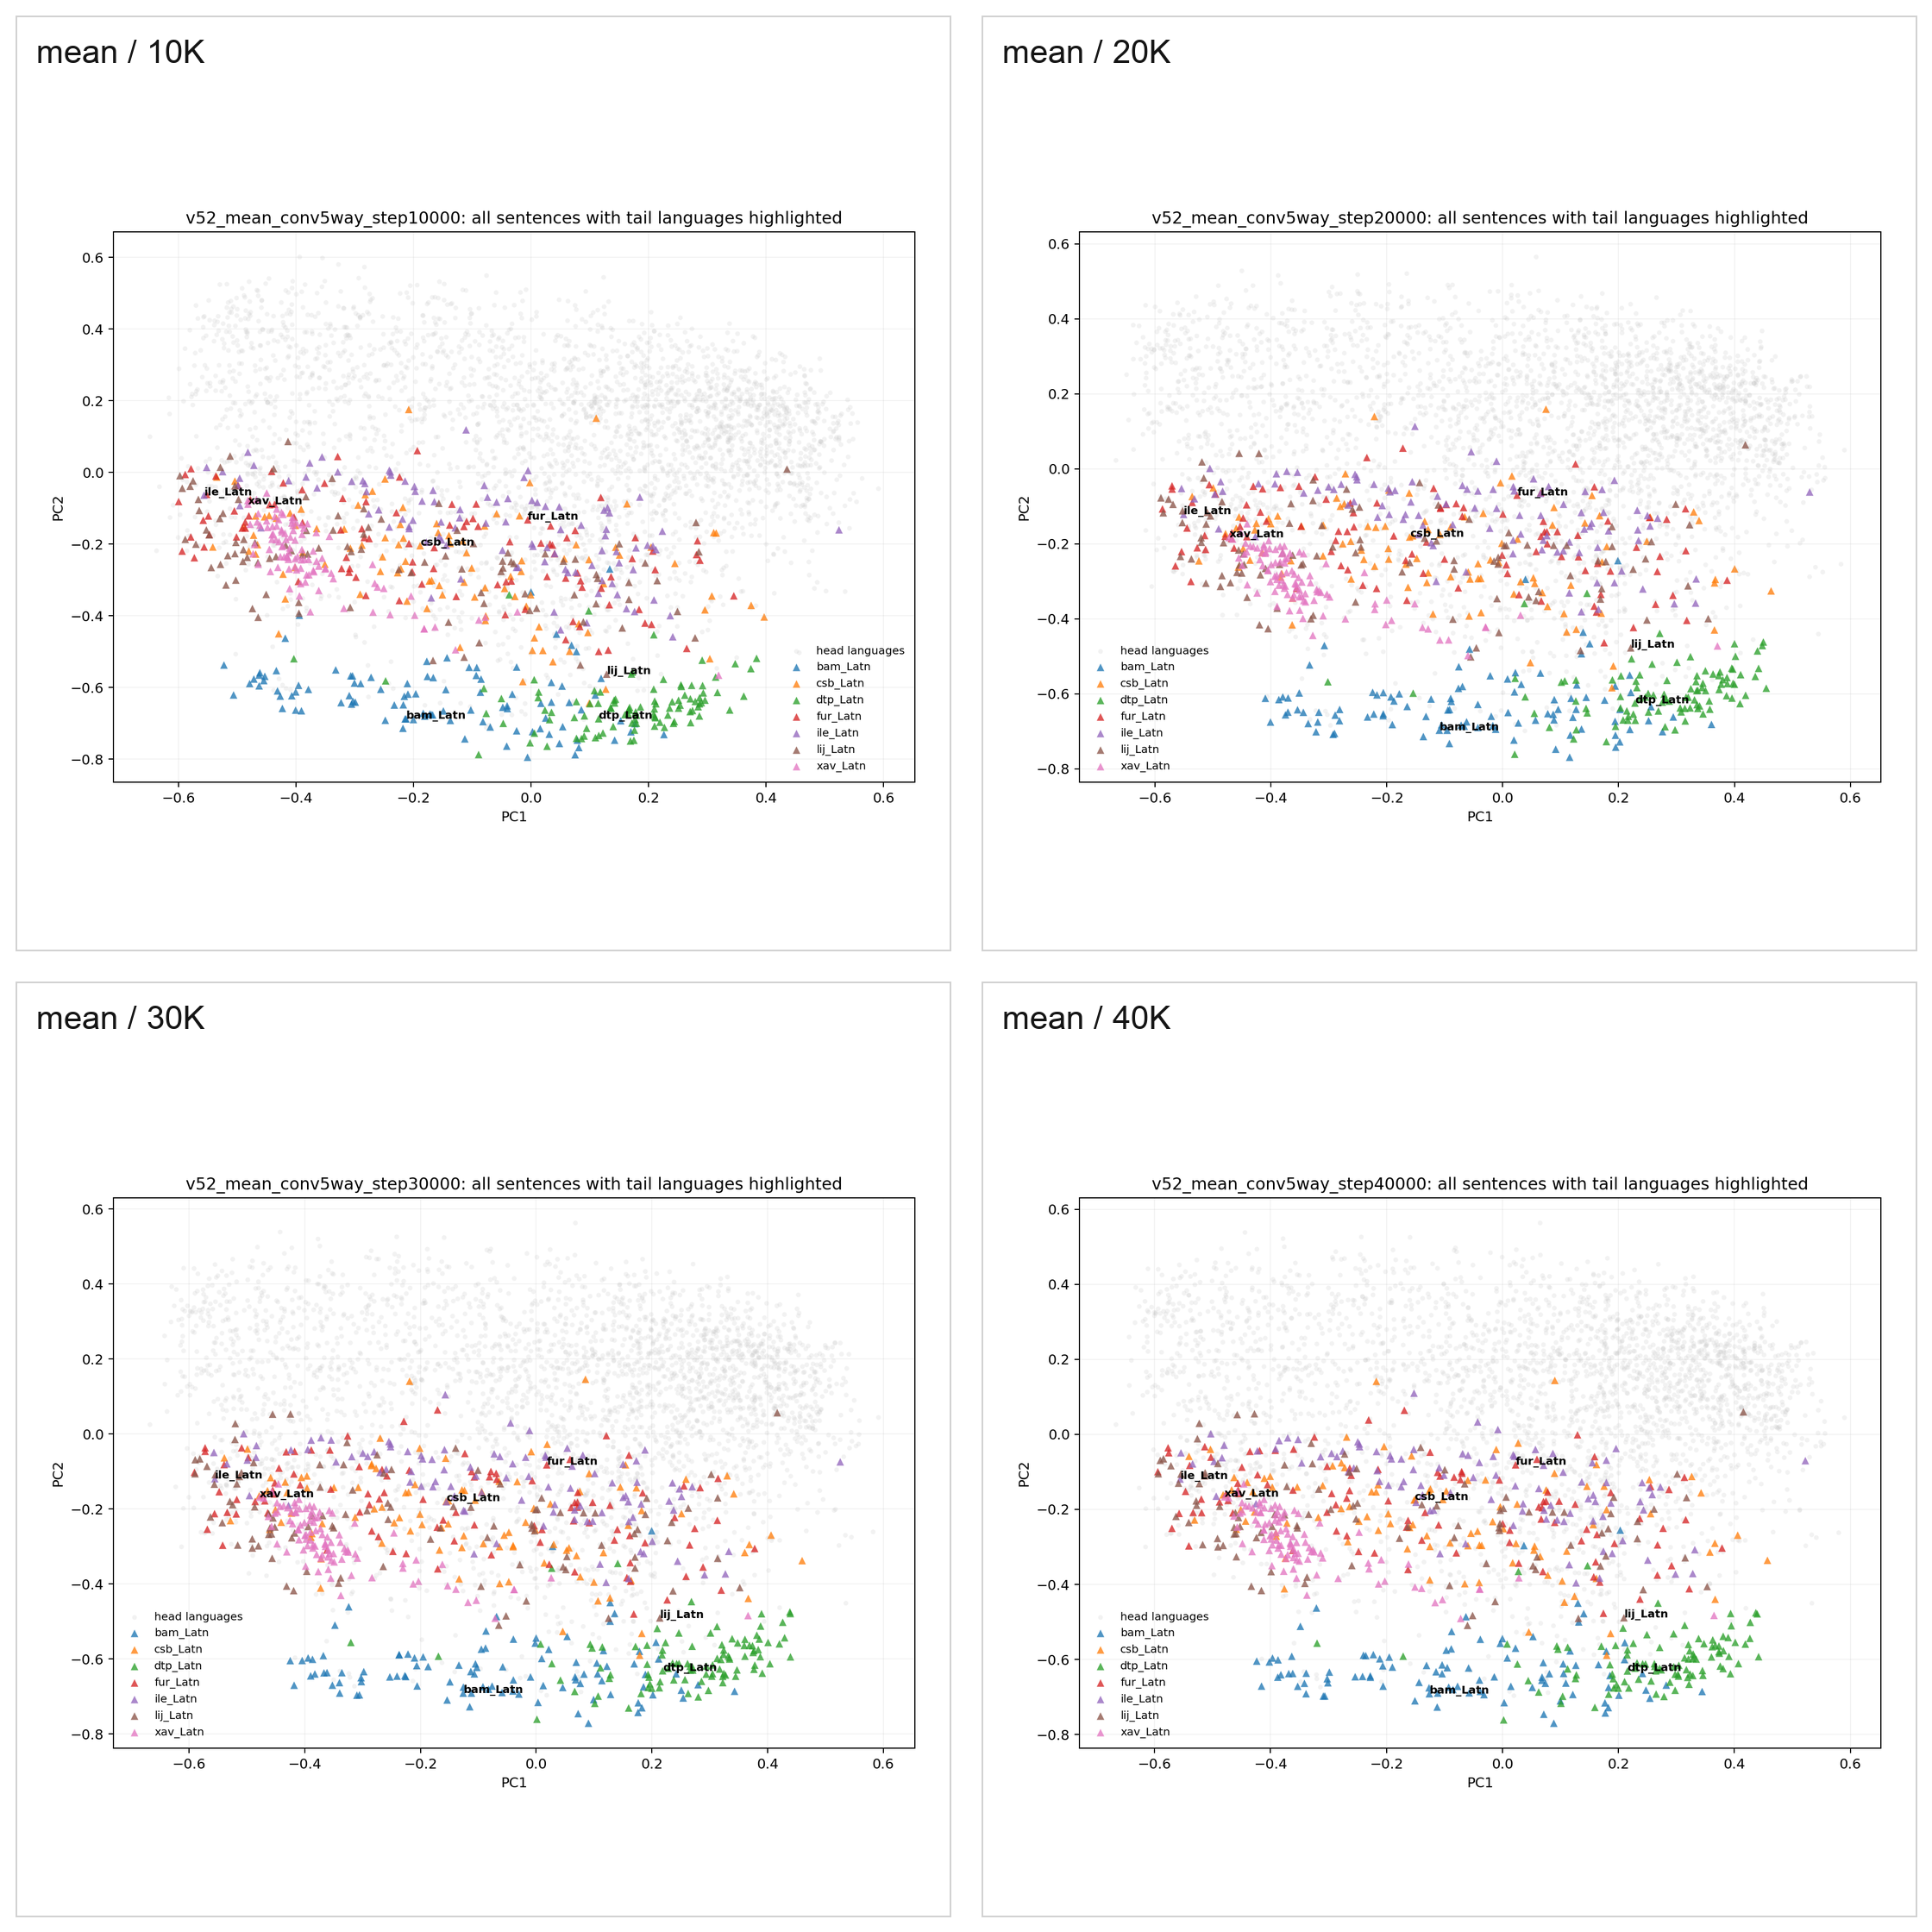
\includegraphics[width=\linewidth]{mapgrid_02.png}
  \caption{Step-by-step 2D maps (2/7): \meanm\ at 10K, 20K, 30K, 40K.}
\end{figure}

\begin{figure}[H]\centering
  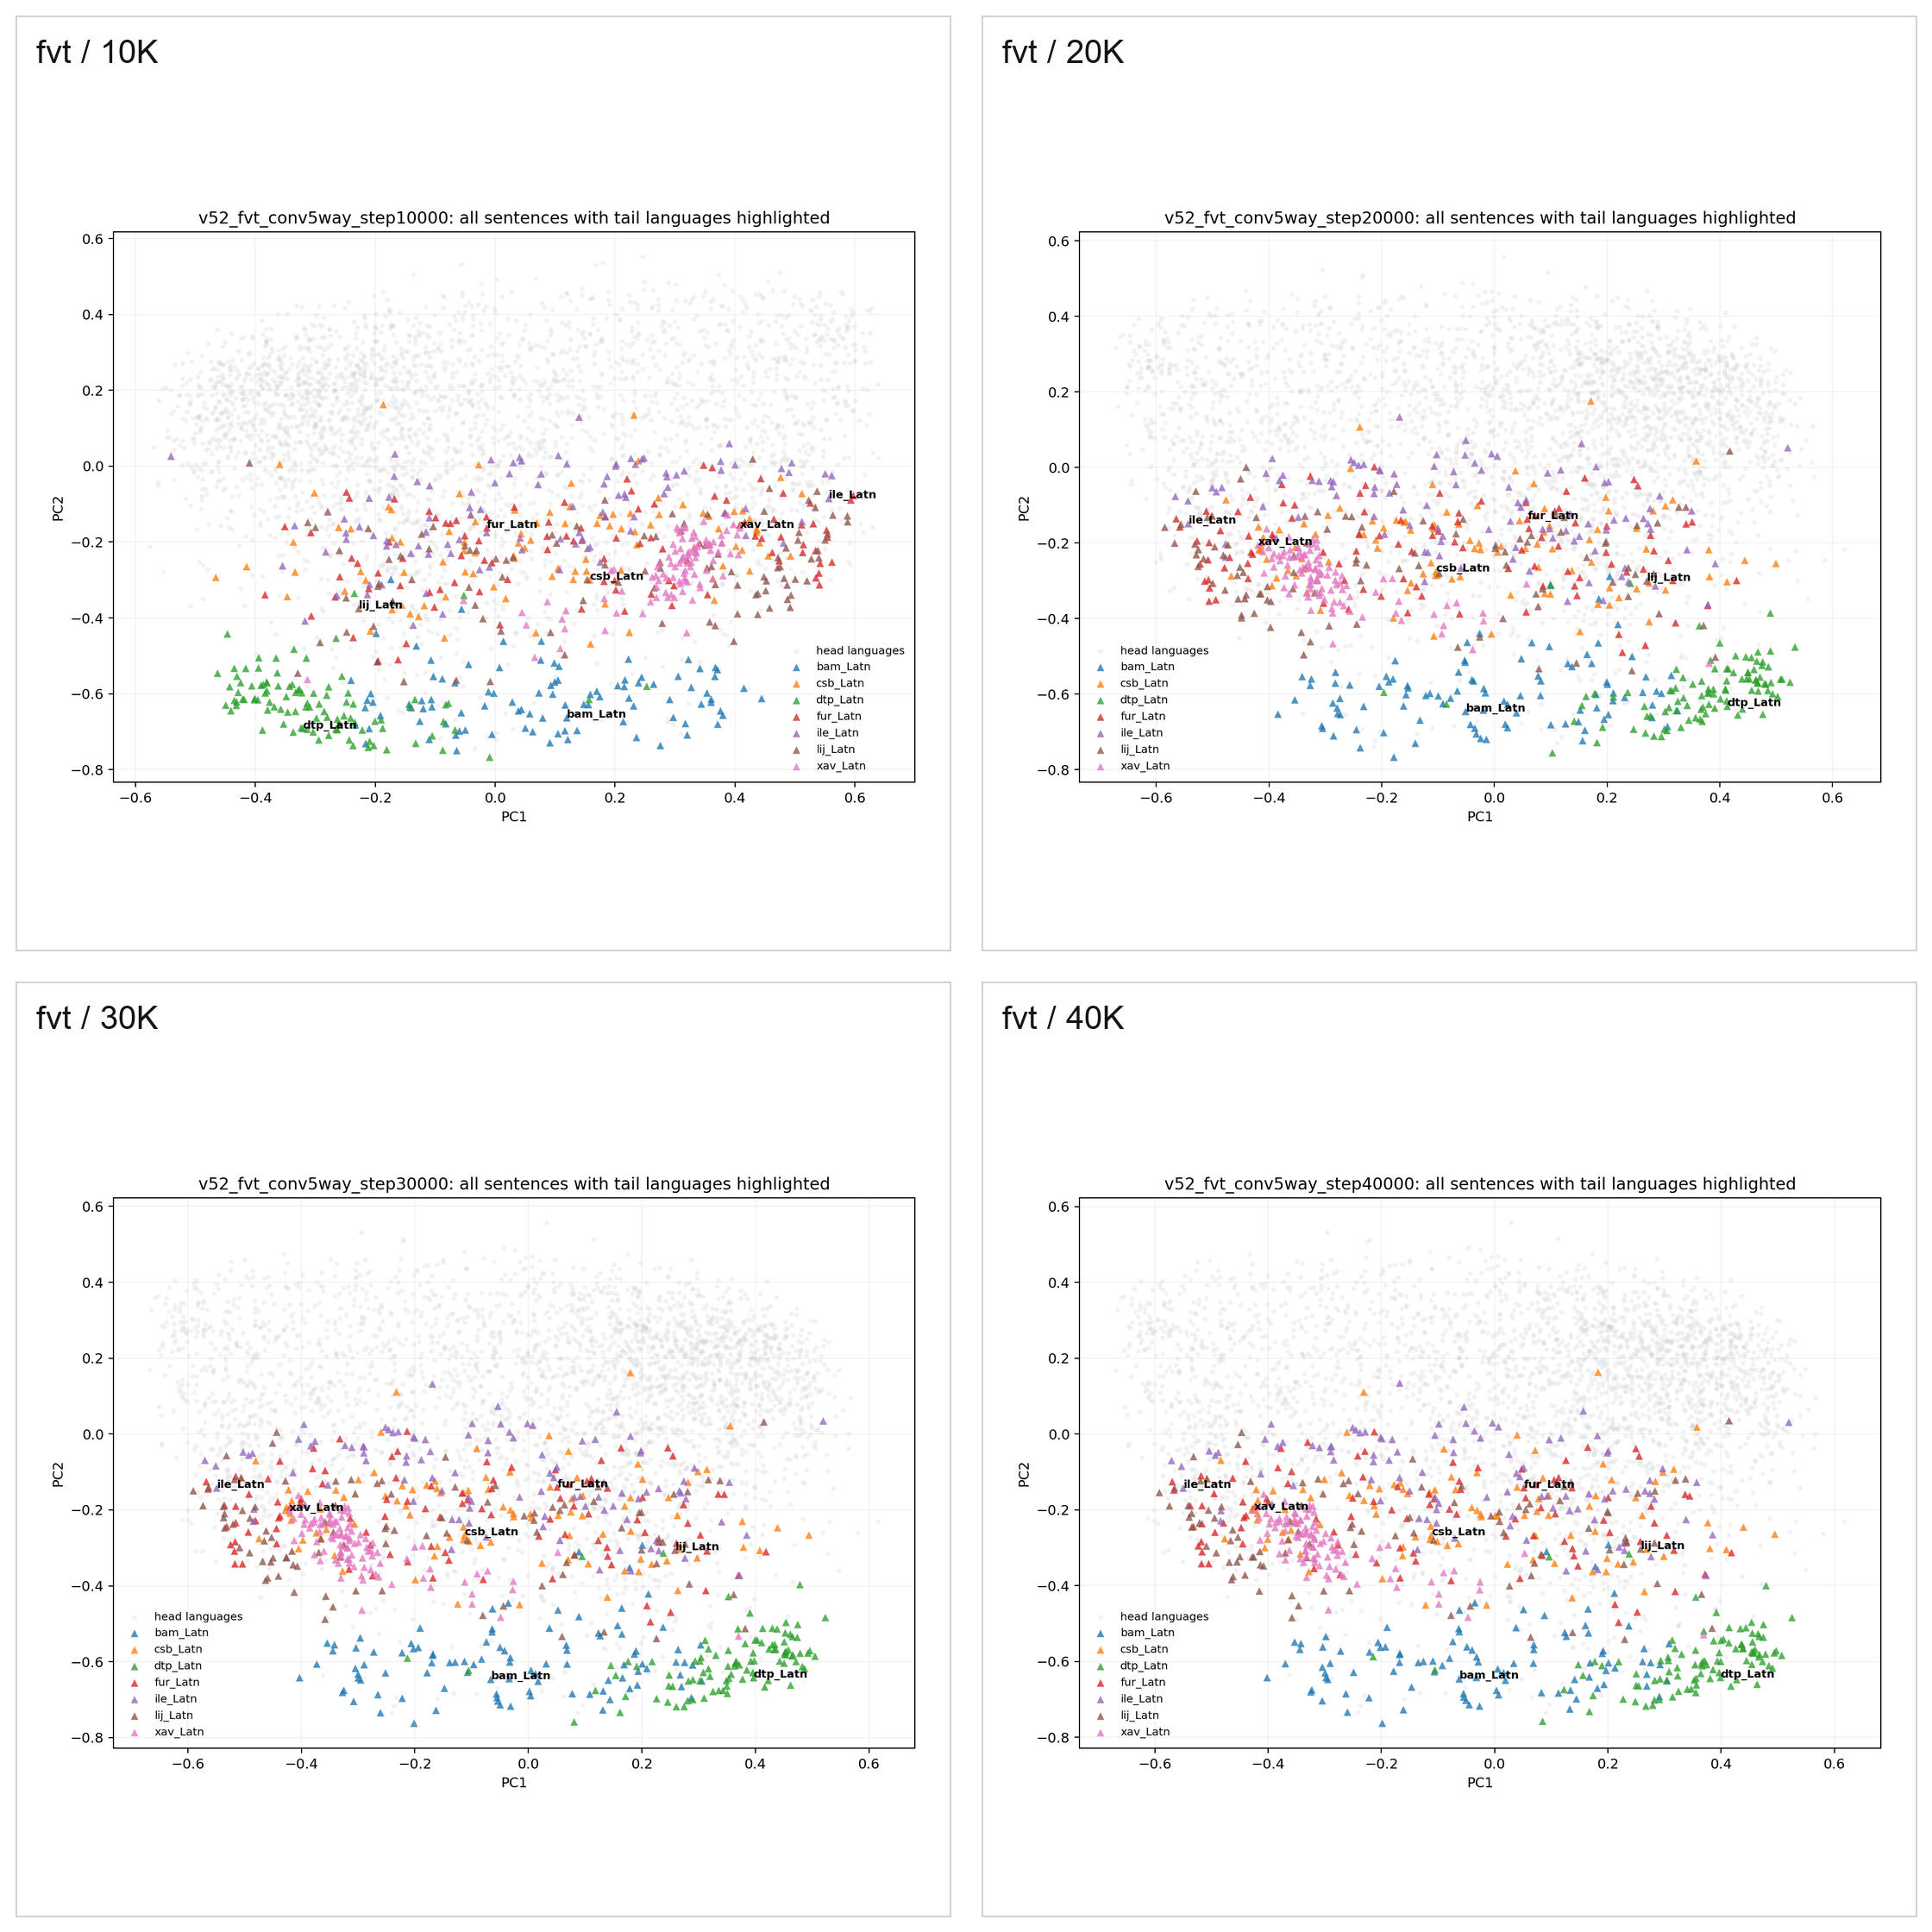
\includegraphics[width=\linewidth]{mapgrid_03.png}
  \caption{Step-by-step 2D maps (3/7): \fvt\ at 10K, 20K, 30K, 40K.}
\end{figure}

\begin{figure}[H]\centering
  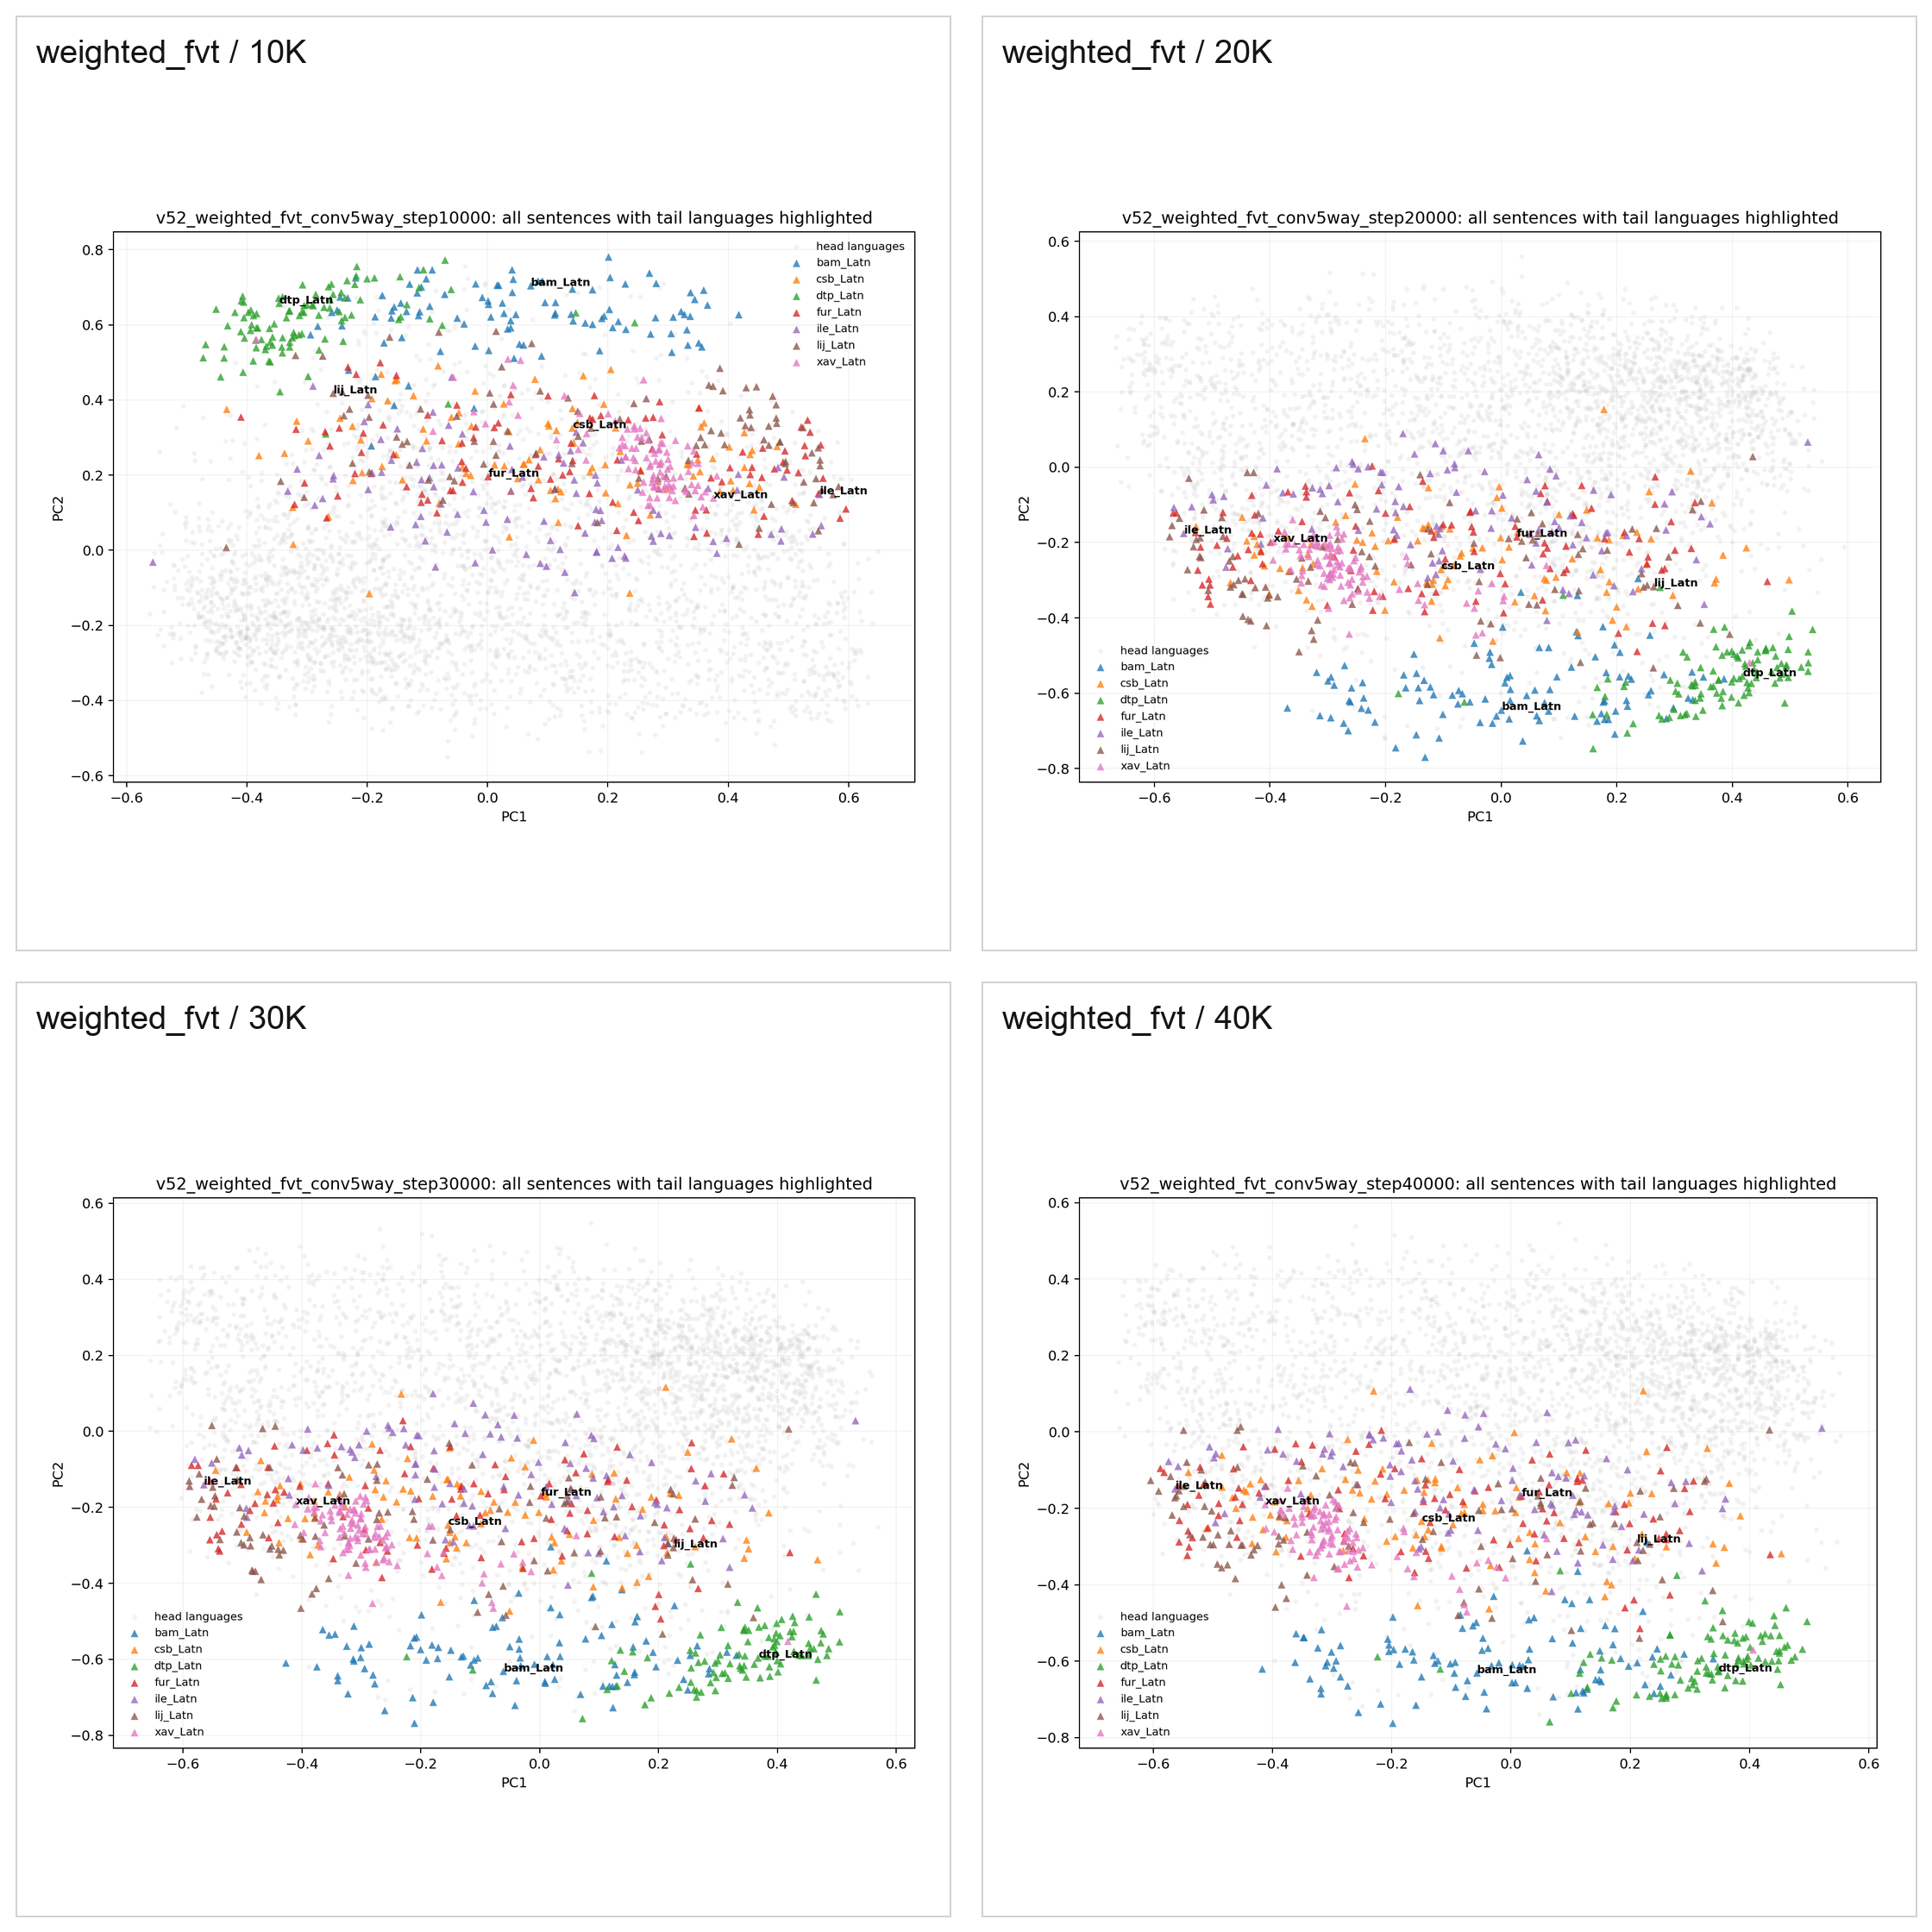
\includegraphics[width=\linewidth]{mapgrid_04.png}
  \caption{Step-by-step 2D maps (4/7): \wfvt\ at 10K, 20K, 30K, 40K.}
\end{figure}

\begin{figure}[H]\centering
  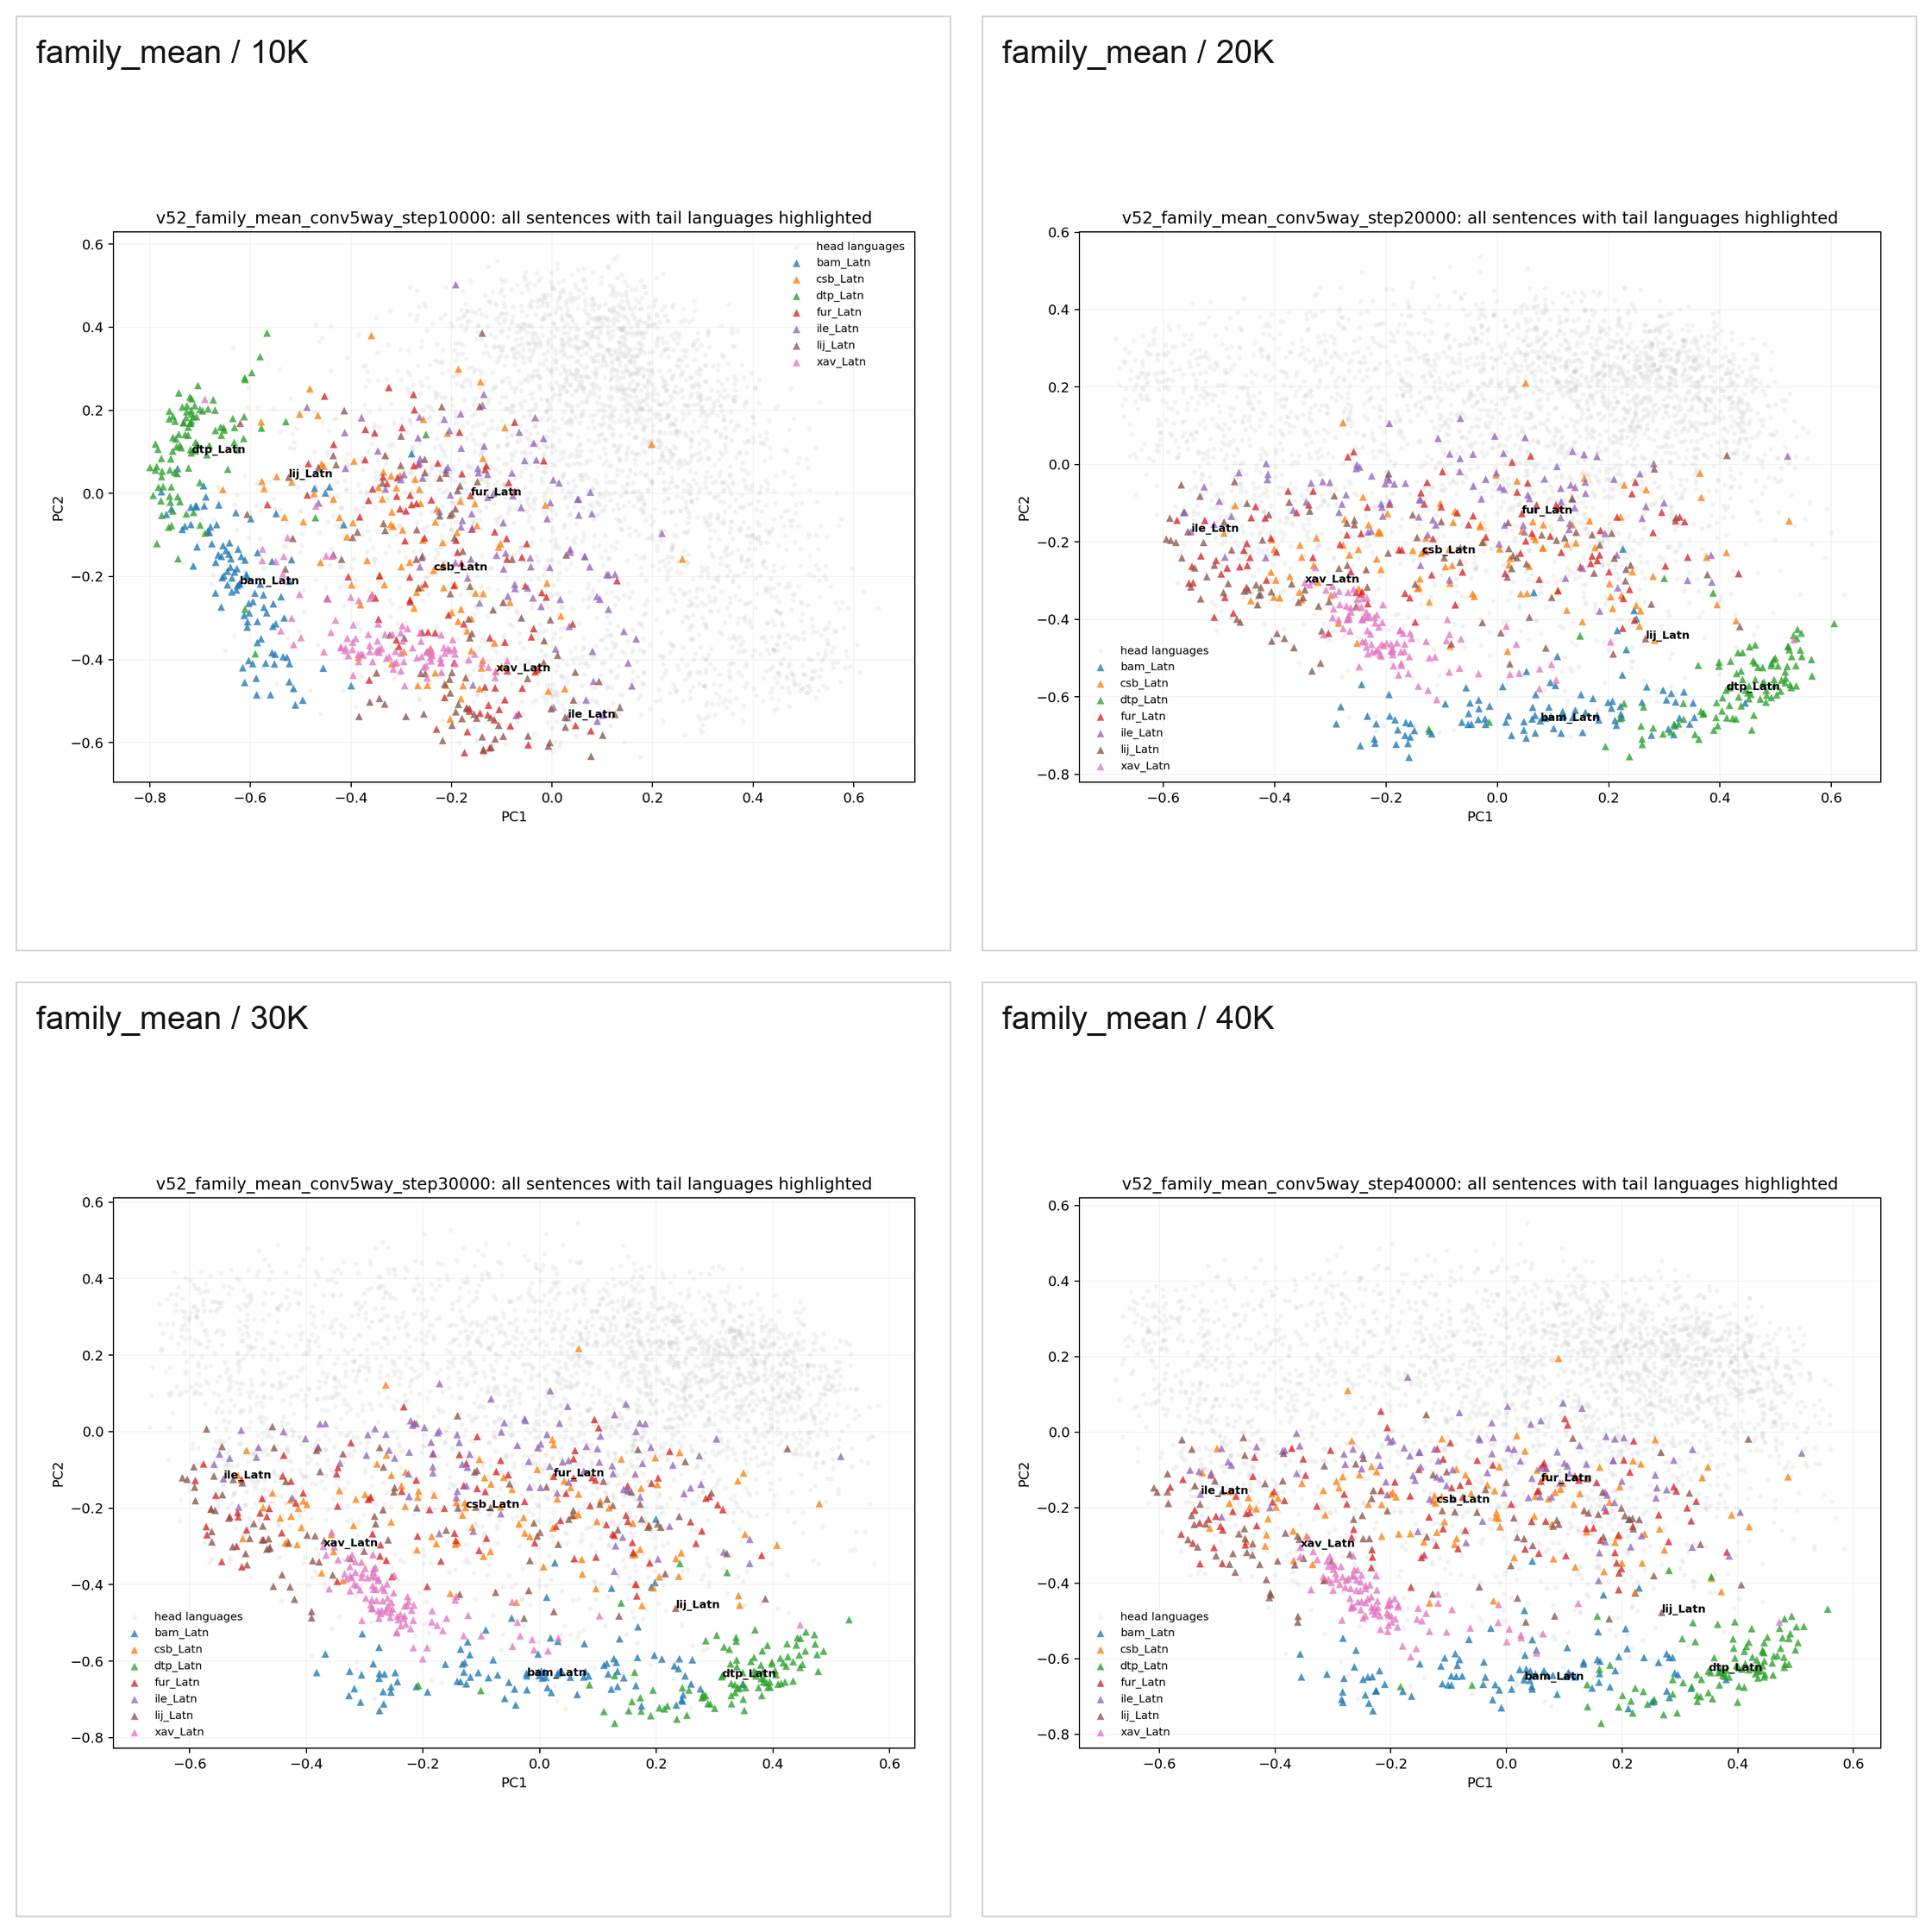
\includegraphics[width=\linewidth]{mapgrid_05.png}
  \caption{Step-by-step 2D maps (5/7): \famm\ at 10K, 20K, 30K, 40K.}
\end{figure}

\begin{figure}[H]\centering
  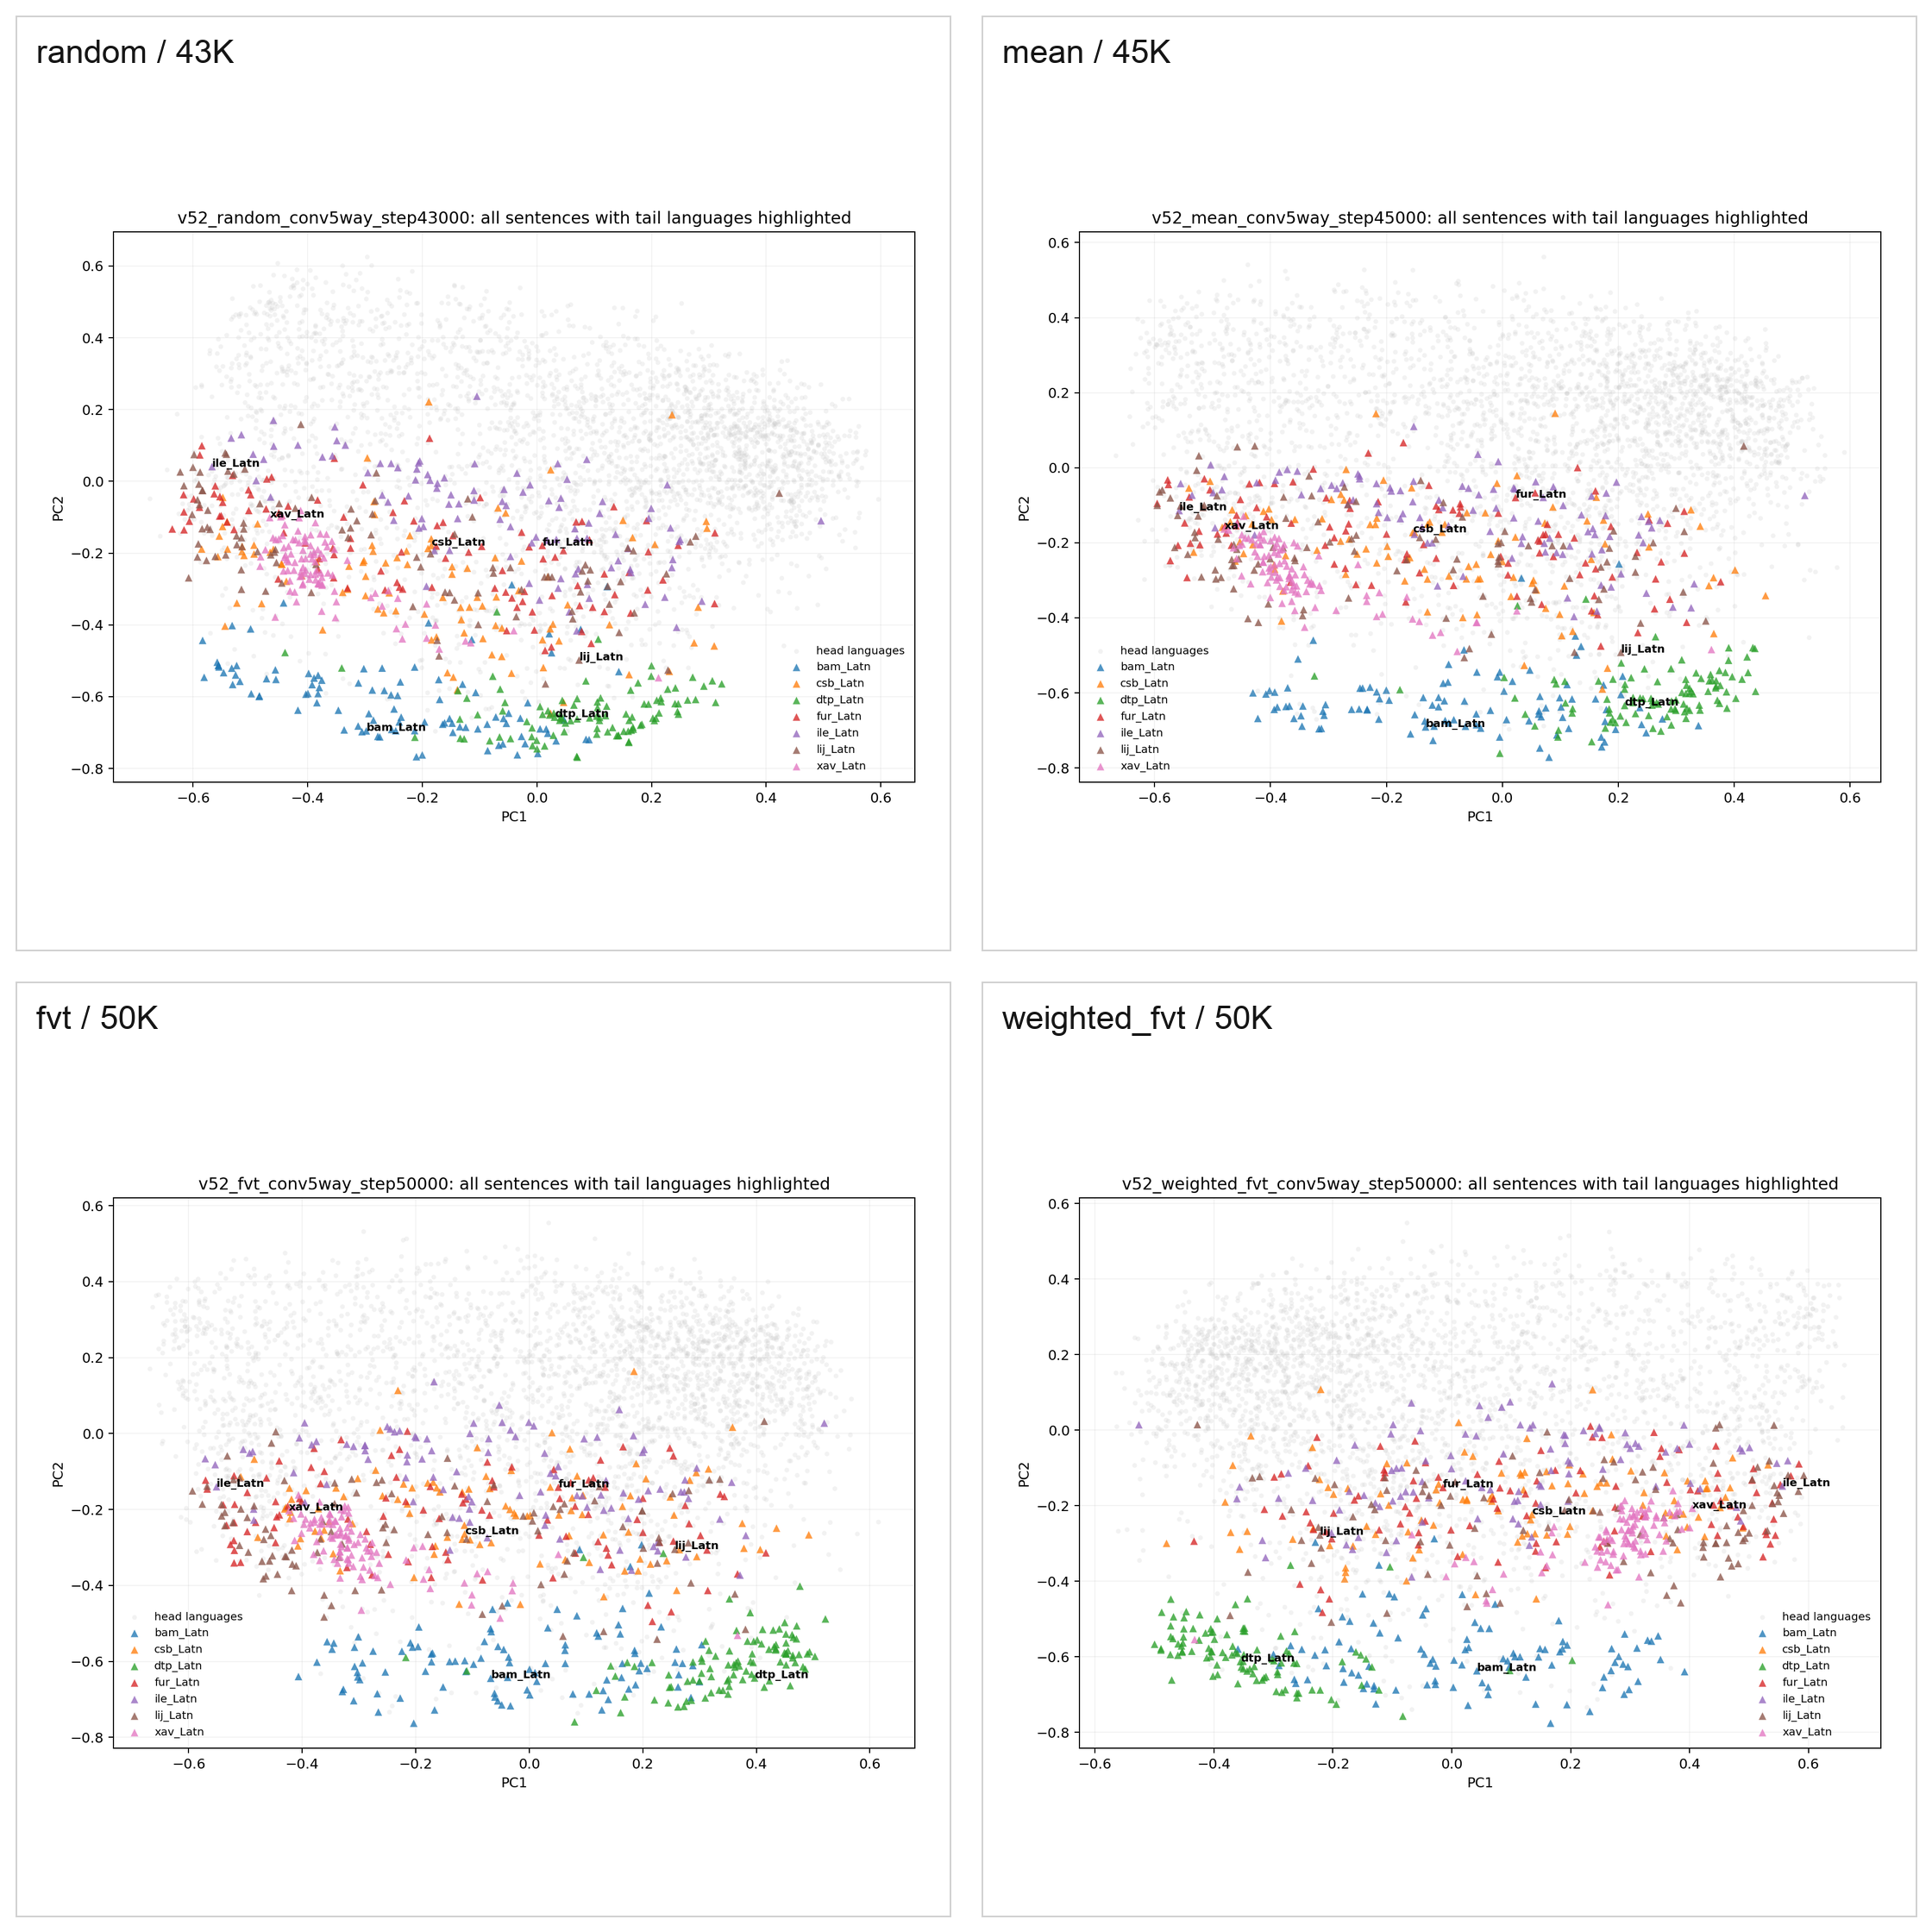
\includegraphics[width=\linewidth]{mapgrid_06.png}
  \caption{Step-by-step 2D maps (6/7): \rand\ 43K, \meanm\ 45K, \fvt\ 50K, \wfvt\ 50K.}
\end{figure}

\begin{figure}[H]\centering
  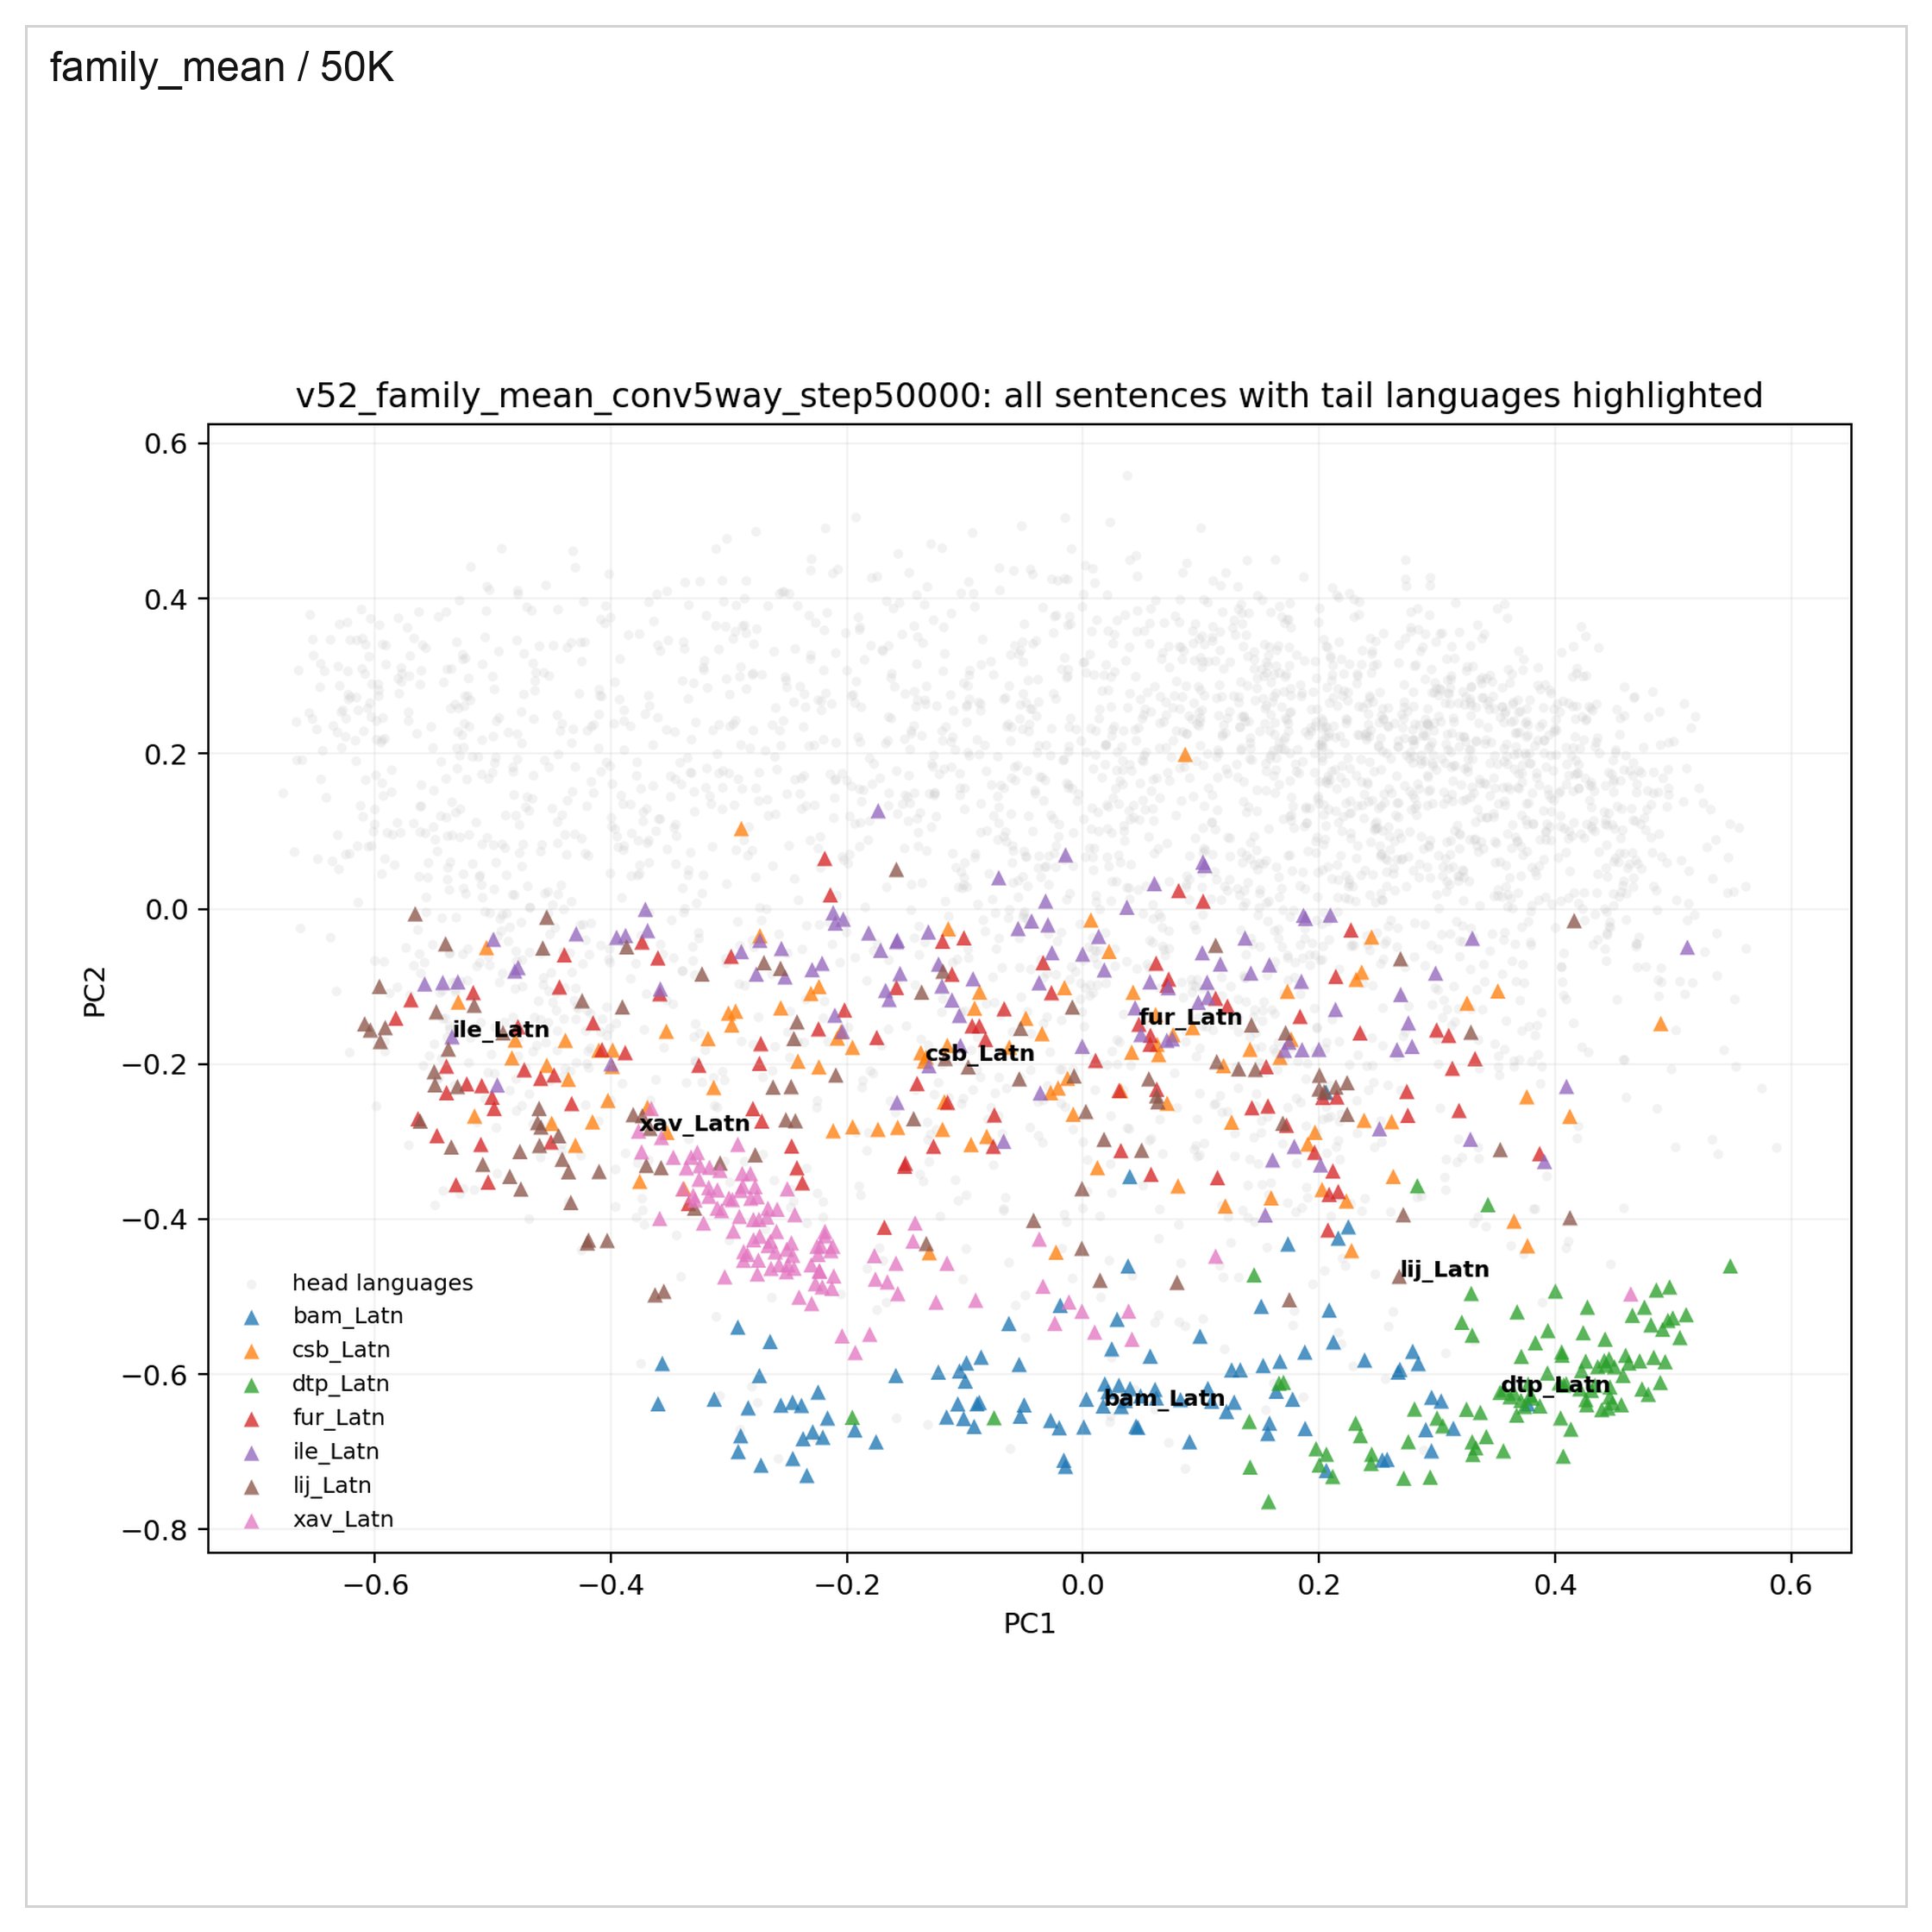
\includegraphics[width=\linewidth]{mapgrid_07.png}
  \caption{Step-by-step 2D maps (7/7): \famm\ 50K.}
\end{figure}

\clearpage
\subsection{38-Language Centroid Map}

Figure~\ref{fig:centroidmap} shows sentence-vector centroids for 38 sampled languages
projected to 2D by PCA at the \fvt\ 50K checkpoint.
Triangles = Target7 tail languages; circles = head/reference languages.

\begin{figure}[H]\centering
  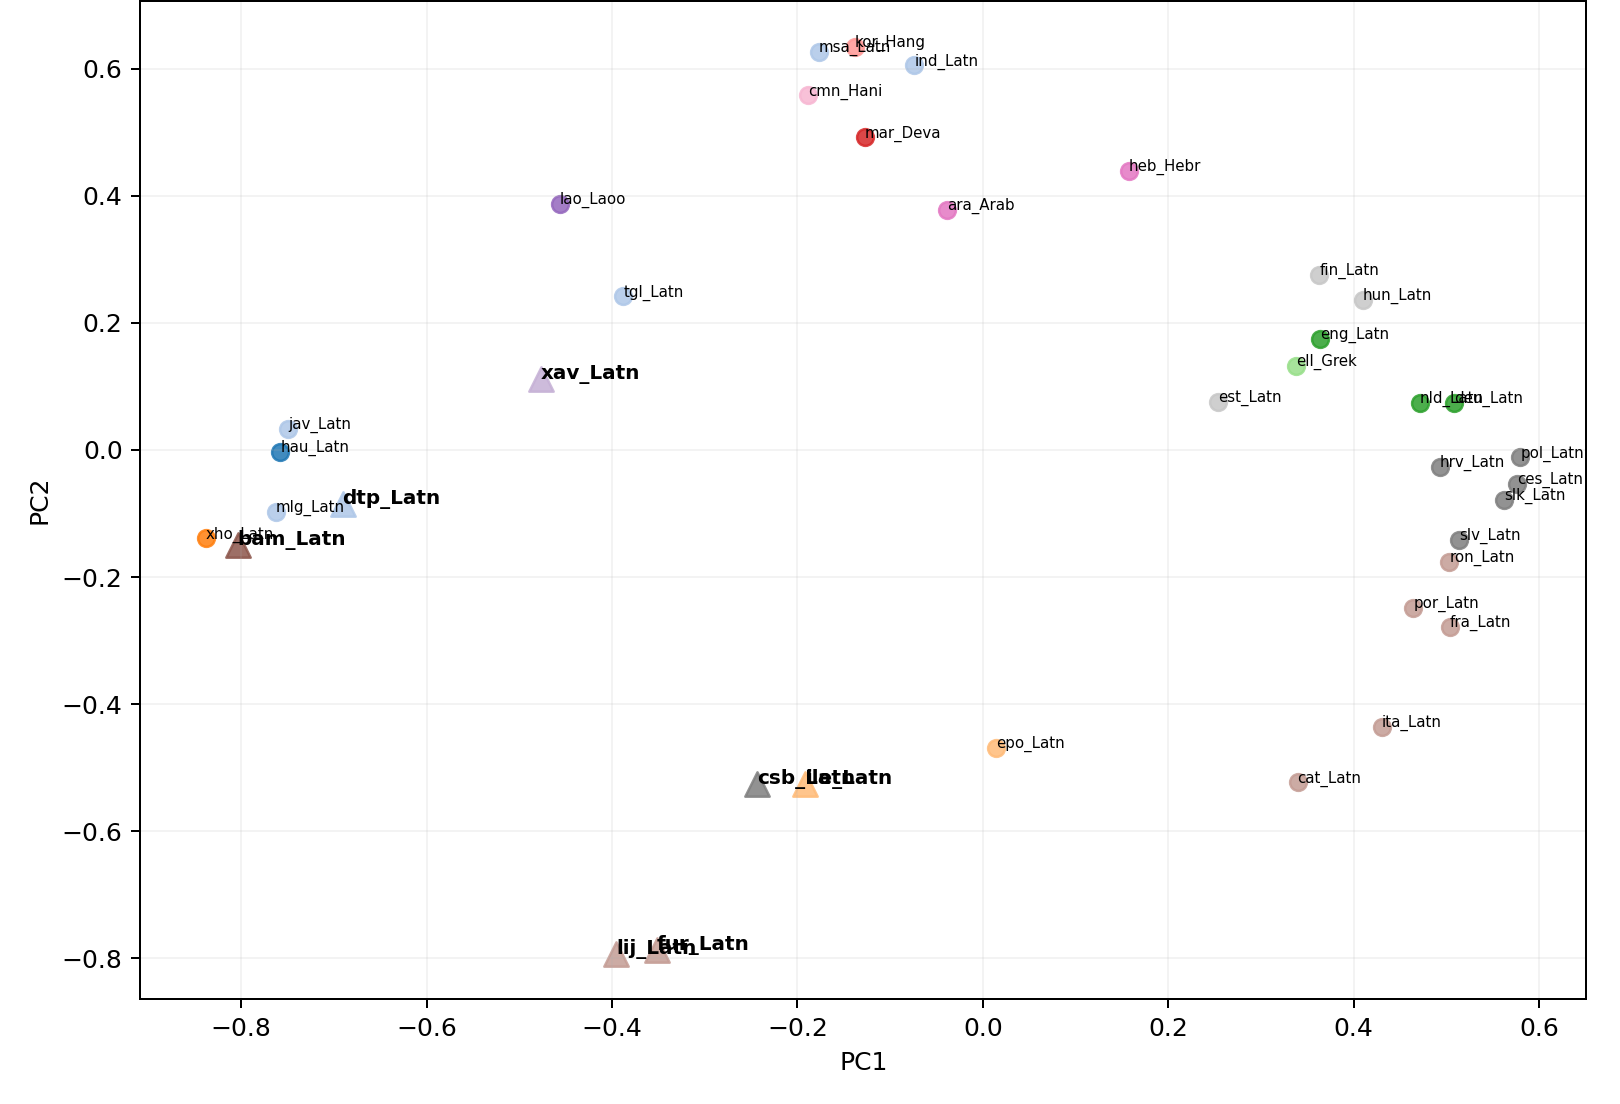
\includegraphics[width=0.88\linewidth]{centroid_fvt_50k.png}
  \caption{2D PCA centroid map for 38 languages (\fvt, 50K).
           Target7 tail languages are shown as triangles;
           head/reference languages as circles.}
  \label{fig:centroidmap}
\end{figure}


\end{document}
